% !TeX encoding = UTF-8
% !TeX program = xelatex
% !TeX spellcheck = en_US

\documentclass[degree=master,degree-type=professional,language=chinese]{ustcthesis}
% degree      = doctor | master | bachelor
% degree-type = academic | professional
% language    = chinese | english
% fontset     = windows | mac | ubuntu | fandol

% https://github.com/zepinglee/gbt7714-bibtex-style/issues/120

\usepackage{ifthen}
% 配置是否为盲审 - use before ustcsetup
\newboolean{BlindReview}
\setboolean{BlindReview}{true} % Set to 'true' or 'false'

% !TeX root = ./main.tex

\ustcsetup{
  title              = {基于神经网络的着色器程序性能预测方法},
  title*             = {Neural network based performance prediction method of shader programs},
  author             = {刘紫檀},
  author*            = {Liu Zitan},
  speciality         = {计算机技术},
  speciality*        = {Computer Technology},
  supervisor         = {陈发来教授, 刘利刚教授},
  supervisor*        = {Prof. Falai Chen, Prof. Ligang Liu},
  % date               = {2017-05-01},  % 默认为今日
  % professional-type  = {专业学位类型},
  % professional-type* = {Professional degree type},
  % department         = {数学科学学院},  % 院系,本科生需要填写
  % student-id         = {PB11001000},  % 学号,本科生需要填写
  % secret-level       = {秘密},     % 绝密|机密|秘密|控阅,注释本行则公开
  % secret-level*      = {Secret},  % Top secret | Highly secret | Secret
  % secret-year        = {10},      % 保密/控阅期限
  % reviewer           = true,      % 声明页显示“评审专家签名”
  %
  % 数学字体
  % math-style         = GB,  % 可选:GB, TeX, ISO
  math-font          = xits,  % 可选:stix, xits, libertinus
}


% 加载宏包

% 定理类环境宏包
\usepackage{amsthm}

% 插图
\usepackage{graphicx}

% 三线表
\usepackage{booktabs}

% 跨页表格
\usepackage{longtable}

% 算法
\usepackage[ruled,linesnumbered]{algorithm2e}

\usepackage{subfigure} % 引入 subfigure 宏包

% SI 量和单位
\usepackage{siunitx}

% 参考文献使用 BibTeX + natbib 宏包
% 顺序编码制
\usepackage[sort]{natbib}
\bibliographystyle{ustcthesis-numerical}

% 著者-出版年制
% \usepackage{natbib}
% \bibliographystyle{ustcthesis-authoryear}

% 本科生参考文献的著录格式
% \usepackage[sort]{natbib}
% \bibliographystyle{ustcthesis-bachelor}

% 参考文献使用 BibLaTeX 宏包
% \usepackage[style=ustcthesis-numeric]{biblatex}
% \usepackage[bibstyle=ustcthesis-numeric,citestyle=ustcthesis-inline]{biblatex}
% \usepackage[style=ustcthesis-authoryear]{biblatex}
% \usepackage[style=ustcthesis-bachelor]{biblatex}
% 声明 BibLaTeX 的数据库
% \addbibresource{bib/ustc.bib}

% 配置图片的默认目录
\graphicspath{{figures/}}

% 数学命令
\makeatletter
\newcommand\dif{%  % 微分符号
  \mathop{}\!%
  \ifustc@math@style@TeX
    d%
  \else
    \mathrm{d}%
  \fi
}
\makeatother
\newcommand\eu{{\symup{e}}}
\newcommand\iu{{\symup{i}}}

% 用于写文档的命令
\DeclareRobustCommand\cs[1]{\texttt{\char`\\#1}}
\DeclareRobustCommand\env{\texttt}
\DeclareRobustCommand\pkg{\textsf}
\DeclareRobustCommand\file{\nolinkurl}

% hyperref 宏包在最后调用
\usepackage{hyperref}


\begin{document}

\maketitle
\copyrightpage

\frontmatter
% !TeX root = ../main.tex

\ustcsetup{
  keywords  = {着色器性能预测, 性能建模, GPU},
  keywords* = {shader performance prediction, performance modeling, GPU},
}

\begin{abstract}
实时渲染技术是计算机图形学技术中的重要组成部分,而实时性是实时渲染永恒追求的主题。故而,在实时图形应用程序开发和优化中,对着色器程序执行时间进行建模和预测的能力至关重要。

GPU 技术的蓬勃发展,让绝大多数实时渲染程序使用了基于可编程着色器的绘制流水线,并通过操作系统提供的图形 API 实现在不同 GPU 设备上的编程。然而,现有的着色器和绘制流水线性能估计方法却受到多种局限:其一,对于厂商提供的性能工具,其提供的性能估计方法通常依赖于厂商提供的、只能适用于自身平台的分析模型和性能计数器;其二,多数工具在着色器程序修改后,均需要重新访问待测平台,在其上进行测试;其三,部分性能分析方法中,只是对指令数量和种类进行简单求和,而没有考虑着色器指令之间上下文关系对性能的影响。

{\amend 为了应对以上挑战,本研究采用数据驱动的方法来解决上述问题。本研究首先构建了一个着色器程序性能数据集,其中包含在 5 个不同平台上总共 54667 个片段着色器性能样本,以用于着色器程序预测模型的训练。为了确保该数据集的可靠性,本研究分析了测得分布的若干特征,同时筛选出了具有挑战性的样本集合。}{\added 为了更好的了解数据集中着色器样本的功能类别特征,本研究还探究了基于基座语言模型的着色器分类标注方案。}

{\amend 本研究随后提出了数据驱动的着色器性能预测方法。相较于现有方法,本研究提出的方法可以更简便的应用到不同 GPU 平台上,并在逐着色器的粒度下提供端到端的性能预测。同时,通过利用神经网络的序列学习能力,GPU 架构特点和程序负载特征等和程序性能相关的因素也加入了考虑,在进一步提高预测准确度的同时使得使用过程中无需再访问待测平台。为了提供更准确的预测,本研究提出了一个单独的 SPIR-V 指令跟踪阶段,用于对着色器程序进行指令编排,并利用编排后着色器程序的运行结果来收集独立于平台的着色器程序跟踪信息,以获得逐 SPIR-V 指令运行计数。除此之外,本研究还}与先前着色器程序性能优化工作中提出的逐指令线性回归方法和简单启发式的两种基线方法相比,本研究的方法将五个平台的平均 MAPE 分别降低了 8.26\% 和 25.25\%,并在所有平台上拥有最佳的 Spearman 相关系数。{\amend 消融和对比实验显示,本研究提出的若干过程和环节对预测器的表现提升均起到了一定程度的帮助。}

  % 摘要分中文和英文两种,中文在前,英文在后,博士论文中文摘要一般 800~1500 个汉字,硕士论文中文摘要一般 500~1000 个汉字。
  % 英文摘要的篇幅参照中文摘要。

  % 关键词另起一行并隔行排列于摘要下方,左顶格,中文关键词间空一字或用分号“,”隔开,英文关键词之间用逗号“,”或分号“;”隔开。

  % 中文摘要是论文内容的总结概括,应简要说明论文的研究目的、基本研究内容、研究方法或过程、结果和结论,突出论文的创新之处。
  % 摘要应具有独立性和自明性,即不用阅读全文,就能获得论文必要的信息。
  % 摘要中不宜使用公式、图表,不引用文献。

  % 中文关键词是为了文献标引工作从论文中选取出来用以表示全文主题内容信息的单词和术语,一般 3~8 个词,要求能够准确概括论文的核心内容。
\end{abstract}

\begin{abstract*}
Real-time rendering technology is a crucial component of computer graphics, and real-time performance is an eternal pursuit in this field. Therefore, the ability to model and predict shader program execution time is essential for the development and optimization of real-time graphics applications.

The rapid development of GPU technology has led to the widespread use of programmable shader-based rendering pipelines in real-time rendering programs, which are implemented on different GPU devices through graphics APIs provided by operating systems. However, existing shader and rendering pipeline performance estimation methods are subject to several limitations. Firstly, performance estimation methods provided by vendor-specific performance tools often rely on proprietary analysis models and performance counters that are only applicable to their own platforms. Secondly, most tools require re-accessing the target platform for testing after modifying shader programs. Thirdly, some performance analysis methods simply sum the number and types of instructions without considering the impact of contextual relationships between shader instructions on performance.

{\amend To address these challenges, this study adopts a data-driven approach. Firstly, a shader program performance dataset is constructed, containing a total of 54,667 fragment shader performance samples across five different platforms, which is used for training shader program prediction models. To ensure the reliability of this dataset, several characteristics of the measured distribution are analyzed, and a set of challenging samples is selected.} To better understand the functional category features of shader samples in the dataset, {\added this study also explores a shader classification annotation scheme based on foundation language models.}

{\amend Subsequently, this study proposes a data-driven shader performance prediction method. Compared to existing methods, the proposed method can be more easily applied to different GPU platforms and provides end-to-end performance prediction at the granularity of individual shaders. By leveraging the sequence learning capabilities of neural networks, factors related to program performance, such as GPU architecture characteristics and program workload features, are also taken into consideration, further improving prediction accuracy while eliminating the need to access the target platform during the usage process. To provide more accurate predictions, this study proposes a separate SPIR-V instruction tracking stage for shader program instruction orchestration and utilizes the execution results of the orchestrated shader programs to collect platform-independent shader program tracing information and obtain per-SPIR-V instruction execution counts.} Additionally, compared to two baseline methods proposed in previous shader program performance optimization work, namely per-instruction linear regression and simple heuristics, the method in this study reduces the average MAPE across five platforms by 8.26\% and 25.25\%, respectively, and achieves the best Spearman correlation coefficient on all platforms. {\amend Ablation and comparative experiments demonstrate that the various processes and components proposed in this study contribute to varying degrees of improvement in the predictor's performance.}
\end{abstract*}

\tableofcontents
% \listoffigures
% \listoftables
% !TeX root = ../main.tex

% \begin{notation}

%   \begin{notationlist}{2em}
%     \item[$\displaystyle a$] The number of angels per unit area
%     \item[$\displaystyle N$] The number of angels per needle point
%     \item[$\displaystyle A$] The area of the needle point
%     \item[$\displaystyle \sigma$] The total mass of angels per unit area
%     \item[$\displaystyle m$] The mass of one angel
%     \item[$\displaystyle \sum_{i=1}^n a_i$] The sum of $a_i$
%   \end{notationlist}

% \end{notation}



% 也可以使用 nomencl 宏包

% \printnomenclature

% \nomenclature{$\displaystyle a$}{The number of angels per unit are}
% \nomenclature{$\displaystyle N$}{The number of angels per needle point}
% \nomenclature{$\displaystyle A$}{The area of the needle point}
% \nomenclature{$\displaystyle \sigma$}{The total mass of angels per unit area}
% \nomenclature{$\displaystyle m$}{The mass of one angel}
% \nomenclature{$\displaystyle \sum_{i=1}^n a_i$}{The sum of $a_i$}


\mainmatter
% % !TeX root = ../main.tex

\chapter{绪论}

\section{研究背景}

\section{挑战与工作重点}

\section{本文结构}


% % !TeX root = ../main.tex

\chapter{浮动体}

\section{三线表}

三线表是《撰写手册》推荐使用的格式,如表~\ref{tab:exampletable}。
\begin{table}[h]
  \centering
  \caption{表号和表题在表的正上方}
  \label{tab:exampletable}
  \begin{tabular}{cl}
    \toprule
    类型   & 描述                                       \\
    \midrule
    挂线表 & 挂线表也称系统表、组织表,用于表现系统结构 \\
    无线表 & 无线表一般用于设备配置单、技术参数列表等   \\
    卡线表 & 卡线表有完全表,不完全表和三线表三种       \\
    \bottomrule
  \end{tabular}
  \note{注:表注分两种,第一种是对全表的注释,用不加阿拉伯数字排在表的下边,
    前面加“注:”;第二种是和表内的某处文字或数字相呼应的注,
    在表里面用带圈的阿拉伯数字在右上角标出,然后在表下面用同样的圈码注出来}
\end{table}

编制表格应简单明了,表达一致,明晰易懂,表文呼应、内容一致。
排版时表格字号略小,或变换字体,尽量不分页,尽量不跨节。
表格太大需要转页时,需要在续表上方注明“续表”,表头页应重复排出。



\section{插图}

有的同学可能听说“\LaTeX{} 只能使用 eps 格式的图片”,甚至把 jpg 格式转为 eps。
事实上,这种做法已经过时。
而且每次编译时都要要调用外部工具解析 eps,导致降低编译速度。
所以我们推荐矢量图直接使用 pdf 格式,位图使用 jpeg 或 png 格式。
\begin{figure}[h]
  \centering
  
\includegraphics[width=0.3\textwidth]{ustc-badge.pdf}
  \caption{图号、图题置于图的下方}
  \label{fig:badge}
  \note{注:图注的内容不宜放到图题中。}
\end{figure}

关于图片的并排,推荐使用较新的 \pkg{subcaption} 宏包,
不建议使用 \pkg{subfigure} 或 \pkg{subfig} 等宏包。



\section{算法环境}

模板中使用 \pkg{algorithm2e} 宏包实现算法环境。关于该宏包的具体用法,
请阅读宏包的官方文档。

\begin{algorithm}[h]
  \SetAlgoLined
  \KwData{this text}
  \KwResult{how to write algorithm with \LaTeX2e }

  initialization\;
  \While{not at end of this document}{
    read current\;
    \eIf{understand}{
      go to next section\;
      current section becomes this one\;
    }{
      go back to the beginning of current section\;
    }
  }
  \caption{算法示例1}
  \label{algo:algorithm1}
\end{algorithm}

注意,我们可以在论文中插入算法,但是插入大段的代码是愚蠢的。
然而这并不妨碍有的同学选择这么做,对于这些同学,建议用 \pkg{listings} 宏包。

% % % !TeX root = ../main.tex

% \chapter{数学}

% \section{数学符号}

% 《撰写手册》要求数学符号遵循 GB/T 3102.11—1993《物理科学和技术中使用的数学符号》
% \footnote{原 GB 3102.11—1993,自 2017 年 3 月 23 日起,该标准转为推荐性标准。}。
% 该标准参照采纳 ISO 31-11:1992 \footnote{目前已更新为 ISO 80000-2:2019。},
% 但是与 \TeX{} 默认的美国数学学会(AMS)的符号习惯有所区别。
% 具体地来说主要有以下差异:
% \begin{enumerate}
%   \item 大写希腊字母默认为斜体,如
%     \begin{equation*}
%       \Gamma \Delta \Theta \Lambda \Xi \Pi \Sigma \Upsilon \Phi \Psi \Omega.
%     \end{equation*}
%     注意有限增量符号 $\increment$ 固定使用正体,模板提供了 \cs{increment} 命令。
%   \item 小于等于号和大于等于号使用倾斜的字形 $\le$、$\ge$。
%   \item 积分号使用正体,比如 $\int$、$\oint$。
%   \item
%     偏微分符号 $\partial$ 使用正体。
%   \item
%     省略号 \cs{dots} 按照中文的习惯固定居中,比如
%     \begin{equation*}
%       1, 2, \dots, n \quad 1 + 2 + \dots + n.
%     \end{equation*}
%   \item
%     实部 $\Re$ 和虚部 $\Im$ 的字体使用罗马体。
% \end{enumerate}

% 以上数学符号样式的差异可以在模板中统一设置。
% 但是还有一些需要用户在写作时进行处理:
% \begin{enumerate}
%   \item 数学常数和特殊函数名用正体,如
%     \begin{equation*}
%       \uppi = 3.14\dots; \quad
%       \symup{i}^2 = -1; \quad
%       \symup{e} = \lim_{n \to \infty} \left( 1 + \frac{1}{n} \right)^n.
%     \end{equation*}
%   \item 微分号使用正体,比如 $\dif y / \dif x$。
%   \item 向量、矩阵和张量用粗斜体(\cs{symbf}),如 $\symbf{x}$、$\symbf{\Sigma}$、$\symbfsf{T}$。
%   \item 自然对数用 $\ln x$ 不用 $\log x$。
% \end{enumerate}

% 模板中使用 \pkg{unicode-math} 宏包配置数学字体。
% 该宏包与传统的 \pkg{amsfonts}、\pkg{amssymb}、\pkg{bm}、
% \pkg{mathrsfs}、\pkg{upgreek} 等宏包\emph{不}兼容。
% 本模板作了处理,用户可以直接使用 \cs{bm}, \cs{mathscr},
% \cs{upGamma} 等命令。
% 关于数学符号更多的用法,参见 \pkg{unicode-math} 宏包的使用说明和符号列表
% \pkg{unimath-symbols}。



% \section{数学公式}

% 数学公式可以使用 \env{equation} 和 \env{equation*} 环境。
% 注意数学公式的引用应前后带括号,建议使用 \cs{eqref} 命令,比如式~\eqref{eq:example}。
% \begin{equation}
%   \hat{f}(\xi) = \int_{-\infty}^\infty f(x) \eu^{-2 \uppi \iu x \xi} \dif x.
%   \label{eq:example}
% \end{equation}

% 多行公式尽可能在“=”处对齐,推荐使用 \env{align} 环境,比如式~\eqref{eq:align_2}。
% \begin{align}
%   a & = b + c + d + e \label{eq:align_1} \\
%     & = f + g. \label{eq:align_2}
% \end{align}



% \section{量和单位}

% 量和单位要求严格执行 GB 3100~3102—1993 有关量和单位的规定。
% 宏包 \pkg{siunitx} 提供了更好的数字和单位支持:
% \begin{itemize}
%   \item 为了阅读方便,四位以上的整数或小数推荐采用千分空的分节方式:\num{55235367.34623}。
%     四位以内的整数可以不加千分空:\num{1256}。
%   \item 数值与单位符号间留适当空隙:\SI{25.4}{mm},\SI{5.97e24}{\kilo\gram},
%     \SI{-273.15}{\degreeCelsius}。 例外:\SI{12.3}{\degree},\ang{1;2;3}。
%   \item 组合单位默认使用 APS 的格式,即相乘的单位之间留一定空隙: \si{kg.m.s^{-2}},
%     也可以使用居中的圆点: \si[inter-unit-product = \ensuremath{{}\cdot{}}]{kg.m.s^{-2}}。
%     GB 3100—1993 对两者都允许,建议全文统一设置。
%   \item 量值范围使用“~”:\SIrange{10}{15}{mol/L}。
%   \item 注意:词头 \textmu{} 不能写为 u,如:\si{umol} 应为 \si{\micro\mole}、\si{\umol}。
% \end{itemize}



% \section{定理和证明}

% 示例文件中使用 \pkg{amsthm} 宏包配置了定理、引理和证明等环境。
% 用户也可以使用 \pkg{ntheorem} 宏包。

% \begin{definition}
%   If the integral of function $f$ is measurable and non-negative, we define
%   its (extended) \textbf{Lebesgue integral} by
%   \begin{equation}
%     \int f = \sup_g \int g,
%   \end{equation}
%   where the supremum is taken over all measurable functions $g$ such that
%   $0 \le g \le f$, and where $g$ is bounded and supported on a set of
%   finite measure.
% \end{definition}

% \begin{assumption}
% The communication graph is strongly connected.
% \end{assumption}

% \begin{example}
%   Simple examples of functions on $\mathbb{R}^d$ that are integrable
%   (or non-integrable) are given by
%   \begin{equation}
%     f_a(x) =
%     \begin{cases}
%       |x|^{-a} & \text{if } |x| \le 1, \\
%       0        & \text{if } x > 1.
%     \end{cases}
%   \end{equation}
%   \begin{equation}
%     F_a(x) = \frac{1}{1 + |x|^a}, \qquad \text{all } x \in \mathbb{R}^d.
%   \end{equation}
%   Then $f_a$ is integrable exactly when $a < d$, while $F_a$ is integrable
%   exactly when $a > d$.
% \end{example}

% \begin{lemma}[Fatou]
%   Suppose $\{f_n\}$ is a sequence of measurable functions with $f_n \geq 0$.
%   If $\lim_{n \to \infty} f_n(x) = f(x)$ for a.e. $x$, then
%   \begin{equation}
%     \int f \le \liminf_{n \to \infty} \int f_n.
%   \end{equation}
% \end{lemma}

% \begin{remark}
%   We do not exclude the cases $\int f = \infty$,
%   or $\liminf_{n \to \infty} f_n = \infty$.
% \end{remark}

% \begin{corollary}
%   Suppose $f$ is a non-negative measurable function, and $\{f_n\}$ a sequence
%   of non-negative measurable functions with
%   $f_n(x) \le f(x)$ and $f_n(x) \to f(x)$ for almost every $x$. Then
%   \begin{equation}
%     \lim_{n \to \infty} \int f_n = \int f.
%   \end{equation}
% \end{corollary}

% \begin{proposition}
%   Suppose $f$ is integrable on $\mathbb{R}^d$. Then for every $\epsilon > 0$:
%   \begin{enumerate}
%     \renewcommand{\theenumi}{\roman{enumi}}
%     \item There exists a set of finite measure $B$ (a ball, for example) such
%       that
%       \begin{equation}
%         \int_{B^c} |f| < \epsilon.
%       \end{equation}
%     \item There is a $\delta > 0$ such that
%       \begin{equation}
%         \int_E |f| < \epsilon \qquad \text{whenever } m(E) < \delta.
%       \end{equation}
%   \end{enumerate}
% \end{proposition}

% \begin{theorem}
%   Suppose $\{f_n\}$ is a sequence of measurable functions such that
%   $f_n(x) \to f(x)$ a.e. $x$, as $n$ tends to infinity.
%   If $|f_n(x)| \le g(x)$, where $g$ is integrable, then
%   \begin{equation}
%     \int |f_n - f| \to 0 \qquad \text{as } n \to \infty,
%   \end{equation}
%   and consequently
%   \begin{equation}
%     \int f_n \to \int f \qquad \text{as } n \to \infty.
%   \end{equation}
% \end{theorem}

% \begin{proof}
%   Trivial.
% \end{proof}

% \newtheorem*{axiomofchoice}{Axiom of choice}
% \begin{axiomofchoice}
%   Suppose $E$ is a set and ${E_\alpha}$ is a collection of
%   non-empty subsets of $E$. Then there is a function $\alpha
%   \mapsto x_\alpha$ (a ``choice function'') such that
%   \begin{equation}
%     x_\alpha \in E_\alpha,\qquad \text{for all }\alpha.
%   \end{equation}
% \end{axiomofchoice}

% \newtheorem{observation}{Observation}
% \begin{observation}
%   Suppose a partially ordered set $P$ has the property
%   that every chain has an upper bound in $P$. Then the
%   set $P$ contains at least one maximal element.
% \end{observation}
% \begin{proof}[A concise proof]
%   Obvious.
% \end{proof}

% % !TeX root = ../main.tex

\chapter{引用文献的标注}

模板使用 \pkg{natbib} 宏包来设置参考文献引用的格式,
更多引用方法可以参考该宏包的使用说明。



\section{顺序编码制}

\subsection{角标数字标注法}

\ustcsetup{
  cite-style = super,
}
\noindent
\begin{tabular}{l@{\quad$\Rightarrow$\quad}l}
  \verb|\cite{knuth86a}|         & \cite{knuth86a}         \\
  \verb|\citet{knuth86a}|        & \citet{knuth86a}        \\
  \verb|\cite[42]{knuth86a}|     & \cite[42]{knuth86a}     \\
  \verb|\cite{knuth86a,tlc2}|    & \cite{knuth86a,tlc2}    \\
  \verb|\cite{knuth86a,knuth84}| & \cite{knuth86a,knuth84} \\
\end{tabular}


\subsection{数字标注法}

\ustcsetup{
  cite-style = inline,
}
\noindent
\begin{tabular}{l@{\quad$\Rightarrow$\quad}l}
  \verb|\cite{knuth86a}|         & \cite{knuth86a}         \\
  \verb|\citet{knuth86a}|        & \citet{knuth86a}        \\
  \verb|\cite[42]{knuth86a}|     & \cite[42]{knuth86a}     \\
  \verb|\cite{knuth86a,tlc2}|    & \cite{knuth86a,tlc2}    \\
  \verb|\cite{knuth86a,knuth84}| & \cite{knuth86a,knuth84} \\
\end{tabular}



\section{著者-出版年制标注法}

\ustcsetup{
  cite-style = authoryear,
}
\noindent
\begin{tabular}{l@{\quad$\Rightarrow$\quad}l}
  \verb|\cite{knuth86a}|         & \cite{knuth86a}         \\
  \verb|\citep{knuth86a}|        & \citep{knuth86a}        \\
  \verb|\citet[42]{knuth86a}|    & \citet[42]{knuth86a}    \\
  \verb|\citep[42]{knuth86a}|    & \citep[42]{knuth86a}    \\
  \verb|\cite{knuth86a,tlc2}|    & \cite{knuth86a,tlc2}    \\
  \verb|\cite{knuth86a,knuth84}| & \cite{knuth86a,knuth84} \\
\end{tabular}

\ustcsetup{
  cite-style = super,
}

% 注意,参考文献列表中的每条文献在正文中都要被引用。这里只是为了示例。
\nocite{*}

% !TeX root = ../main.tex

\chapter{绪论}

\section{研究背景}

作为计算机图形学的一个分支,渲染是将用不同表达表示的几何、材质、光照、相机等信息综合,然后最终生成二维图像的过程。根据一幅图像渲染时间来分类,计算机图形学领域通常将渲染技术分为实时渲染和离线渲染两个大类。对于实时渲染来说,实时性是需要保证的重要性能指标,而这一般意味着绘制帧率需要达到每秒 30 幅画面或更高。

利用专用的 GPU 和光栅化图形管线来进行实时渲染是目前的主流方案。这种方案将实时渲染过程抽象为以顶点输入,顶点着色,光栅化,片段着色和深度模板测试为阶段的管线过程。为了方便对不同厂商生产的 GPU 进行编程,设备和操作系统厂商间约定了比较稳定的图形 API,例如现在由 Khronos Group 负责的 OpenGL,OpenGL ES,Vulkan,由 Microsoft 公司负责的 Direct3D 和由 Apple 负责的 Metal 等。

早期的图形管线设计多以固定管线功能为主,图形程序员只能够操作管线功能的开启和关闭,并不能像自己编写程序一样对顶点和片段颜色等进行管线预设功能之外的操作。随着图形硬件的功能演进,OpenGL 和 Direct3D 均加入了通过图形程序员编写的专用程序片段来替换部分固定管线的实现的功能。这样的专用程序片段被称为着色器程序 (Shader Program)。

对于现代图形 API 来说,着色器程序本身以 HLSL,GLSL 等高层次描述语言写就,并在程序运行时呈递给设备厂商或操作系统厂商提供的驱动程序中的编译器进行运行时编译。多种多样的着色器程序极大的丰富了光栅化图形管线可以实现的图形和图像效果,成为了现在游戏、VR 等交互式互动娱乐应用程序编写时的重要组成部分。

为了适应实时渲染在各种类型终端上的广泛需求, GPU 市场十分丰富。对于桌面端,就有 Intel, AMD, NVIDIA, Apple 等公司提供 GPU 解决方案;而如 Qualcomm,Broadcom,Imagination,华为等公司则提供移动端的 GPU 和 IP 解决方案。这些 GPU 家族,包括其各自每代的处理器设计,通常拥有不同的指令集架构 (Instruction Set Architecture, ISA),微架构等,而仅仅在图形 API 的层次上做到对使用者一致。例如,桌面端的 GPU 普遍支持 Direct3D,Vulkan,OpenGL 等图形 API,移动端的 GPU 则普遍支持 OpenGL ES, Vulkan 等图形 API。对于应用开发者来说,设备厂商通过图形 API 层来努力隔离设备之间的异质性。

然而,这种隔离并不是充分的。不同的架构和单元配置会影响 GPU 执行用户负载时的性能,而这种性能上的区别会对最终用户的体验产生或多或少的影响。在所有图形程序的性能影响因素中,着色器程序因其可编程性,会对性能产生较大的影响。因此,本文围绕着光栅化图形管线中的着色器程序,研究其性能的预测问题。

\section{挑战与研究内容}

针对于 GPU 上应用的性能预测和优化问题,业界已经开发出多种工具和方法。以 Radeon Graphics Profiler\cite{AMDRGP} 和 NSight Graphics\cite{NSightGraphics} 为例,它们会通过一次或多次专门的管线性能剖析过程,利用 GPU 内部的性能计数器给出着色器的优化建议。此外,诸如 Emerald 和 GPGPU-Sim 这样的体系结构模拟器,则通过对 GPU 架构的模拟和较精确的建模来预测着色器的性能。然而,上述方法和工具的局限性在于,其依赖于特定的厂商或 GPU 架构,且需要在每一种 GPU 上进行单独测试或专门的模拟运行。这样一来,在高度分散的 GPU 市场中,这种特性要求开发者对每一种平台都进行单独的建模或性能分析,增加了额外的测试和调优负担。

在着色器优化和简化问题过程中,学术界曾有相关研究对待优化的着色器性能进行建模。然而,这些工作主要采用较简单的性能估算方法,比如认为着色器的运行时间和着色器中进行的标量运算以及纹理访问操作次数成正比。然而,着色器指令的执行时间受到多种因素的影响。这些影响因素包括编译器优化和 GPU 架构特点,如缓存系统设计和运算单元的数量等。因此,这些未能充分考虑这些因素的模型,往往不能准确预测性能表现。

基于上面的观察,本文主要提出了一种利用神经网络,针对不同 GPU 平台上图形管线中着色器的性能进行建模和预测的方法。利用基于神经网络的学习方法,本文提出的方法可以较为简便的应用到不同 GPU 平台上,达到平台无关性。同时,通过利用神经网络对着色器程序进行学习, GPU 架构特点和程序负载特征等和程序性能相关的因素也被考虑了进来,从而可以进一步的提高预测准确度。

具体来看,为了对本文提出的方法进行验证,我们收集了来自 Shadertoy 的 27911 个着色器程序,在五个平台收集了总计 54667 个性能样本,并将其作为我们的着色器程序性能数据集。同时,本文所述的方法还实现了在 SPIR-V 着色器中间表示上插桩,从而获得每个 SPIR-V 指令的执行计数,并作为上下文信息输入预测器。同时,为了将程序中的指令作为一个序列整体加以考虑,本文所属的预测方法采用 Transformer 编码器来进行序列学习。

\section{章节安排}

本文的章节安排大致如下:

第一章主要介绍本研究的研究背景、研究意义,挑战和研究的大致内容。

第二章主要介绍本研究相关的背景知识。本研究主要和着色器程序优化,程序语言理解和程序性能建模三个方面相关。

第三章主要介绍本研究提出的,基于神经网络的着色器程序性能预测方法。该章首先给出本方法的总览,随后分别介绍本方法较核心的三部分的设计,分别为着色器程序性能数据集的程序收集、测量和评估方法,基本块粒度的 SPIR-V 指令追踪的程序编排和实现,以及本方法提出的神经网络性能模型。最后,本章给出了上面提到的部分的分析和验证实验。

第四章给出了本研究的工作总结和展望。
% !TeX root = ../main.tex

\chapter{相关工作}

\section{着色器程序优化}

\subsection{GPU 上的实时渲染}

\label{sec:realtime_rendering_in_gpu}

所谓渲染,即是利用计算机程序根据场景中的几何、光照、材质、相机等描述来生成图像的一个过程。根据对真实感的要求以及预期的计算时间开销两个维度,渲染又可以分为离线渲染和实时渲染两大类别。其中,离线渲染往往追求真实的材质、光照表现,而实时渲染则更侧重于画面生成时间的实时性。

% https://en.wikipedia.org/wiki/Geometry_pipelines
% https://www.electronicdesign.com/technologies/embedded/article/21149941/jon-peddie-research-geometry-engine-the-legendary-chip-that-launched-sgi
% https://www.slideshare.net/Mark_Kilgard/sigraph-asia-2008-modern-opengl-presentation#13
% https://dl.acm.org/doi/10.1145/166117.166131 RealityEngine Graphics (SIGGRAPH'93)
% https://www.computer.org/publications/tech-news/chasing-pixels/yamahas-ygy611-a-pioneer-3d-chip
% https://www.computer.org/publications/tech-news/chasing-pixels/1986-ncr-7300 (2d palette only)
% https://www.computer.org/publications/tech-news/chasing-pixels/famous-graphics-chips-hps-artist-graphics
% https://en.wikipedia.org/wiki/Graphics_processing_unit

从算法的角度来看,渲染任务是一个高度并行的计算密集任务,而拥有庞大的分支预测、乱序执行、超标量功能的 CPU 并不天然适合这种任务。在对更高的渲染性能的追求下,适应各种渲染任务或子任务的图形加速器产品应运而生。

早期的图形加速产品通常支持顶点变换、视窗裁剪、透视和正交投影变换,以及直线和样条曲线的生成功能,如 1982 年 SGI 公司的 Geometry Engine \cite{GeometryEngineSGI} 协处理器即为此类产品的范例之一;90 年代中期的产品则多加入着色功能,以支持向多边形图元进行着色,并支持纹理采样、深度缓冲和深度剔除等功能,如 1993 年 SGI 公司的 RealityEngine Graphics \cite{RealityEngineSGI}。图 \ref{fig:reality_engine_graphics} 给出了 RealityEngine Graphics 产品的架构图。可以看到,当时用于交互艺术创作的图形工作站产品已经具有顶点变换、片元生成,以及在片元着色阶段进行纹理采样和多重采样抗锯齿。值得一提的是,这里的“图形流水线”是通过多个 ASIC 拼成的多块板卡实现的,并且可以实现部分的重配置,以适应不同档次的产品所对应的顶点和纹理填充率需求。将绘制流水线中涉及到的多种环节集成到一个 ASIC (专用集成电路)中的 3D 图形处理器,如 1995 年 NVIDIA 公司的 NV1 \cite{NV1NVIDIA, NV1NVIDIANews} 等,则尚不支持硬件加速的顶点变换,而只支持光栅化和后续的着色过程。

随着技术进步和互动娱乐产业的蓬勃发展,图形处理器也逐渐加入了更多功能。例如,2001 年 NVIDIA 公司的 NV20 实现了可编程的顶点变换引擎\cite{10.1145/383259.383274},其可以允许用户在顶点着色阶段传入自定义的着色器程序,而非仅能使用固定管线中有限的功能组合。

截至目前,现在的 GPU 及其对应的 API 接口多支持以图 \ref{fig:rasterize_pipeline} 为基础的光栅化绘制流水线,用于进行 GPU 参与的实时渲染。从图 \ref{fig:rasterize_pipeline} 中可以看到,输入的图元会经历顶点变换、曲面细分、几何着色、光栅化和像素着色阶段,最后在输出合并器 (Output Merger)处将渲染目标(Render Target)送入显存。在这其中,蓝色矩形表示的着色器部分均为可编程着色器部分,可以由程序员经由着色器程序设计语言来编写着色器程序,从而实现自定义的流水线功能。同时,着色器中还可以引用来自显存的其它资源,如纹理、存储缓冲区等 UAV (Unordered Access View)资源。

% \begin{figure}
%     \centering

% \begin{tikzpicture}[node distance=2cm]

% % 定义节点样式
% \tikzstyle{process} = [rectangle, minimum width=4cm, minimum height=1cm, text centered, draw=black]
% \tikzstyle{process2} = [rectangle, minimum width=4cm, minimum height=1cm, text centered, draw=black, rounded corners=.8ex, fill=blue!20]

% % 定义节点
% \node (vertex) [process2] {顶点变换};
% \node (tcs) [process2, below of=vertex] {TCS, 细分着色, TES};
% \node (geometry) [process2, below of=tcs] {几何着色};
% \node (view) [process, below of=geometry] {透视变换};
% \node (clipping) [process, below of=view] {视口裁剪, 背面剔除};
% \node (raster) [process, right = 2cm of clipping] {光栅化};
% \node (earlyZ) [process2, above of=raster] {Early Z, 片段着色};
% \node (zalpha) [process, above of=earlyZ] {深度测试, Alpha混合};
% \node (aa) [process, above of=zalpha] {反走样};
% \node (output) [process, above of=aa] {输出到后端缓冲};

% % 定义箭头
% \draw [->] (vertex) -- (tcs);
% \draw [->] (tcs) -- (geometry);
% \draw [->] (geometry) -- (view);
% \draw [->] (view) -- (clipping);
% \draw [->] (clipping) -- (raster);
% \draw [->] (raster) -- (earlyZ);
% \draw [->] (earlyZ) -- (zalpha);
% \draw [->] (zalpha) -- (aa);
% \draw [->] (aa) -- (output);

% \end{tikzpicture}

%     \caption{光栅化绘制流水线}
%     \label{fig:rasterize_pipeline}
% \end{figure}

\begin{figure}
    \centering
    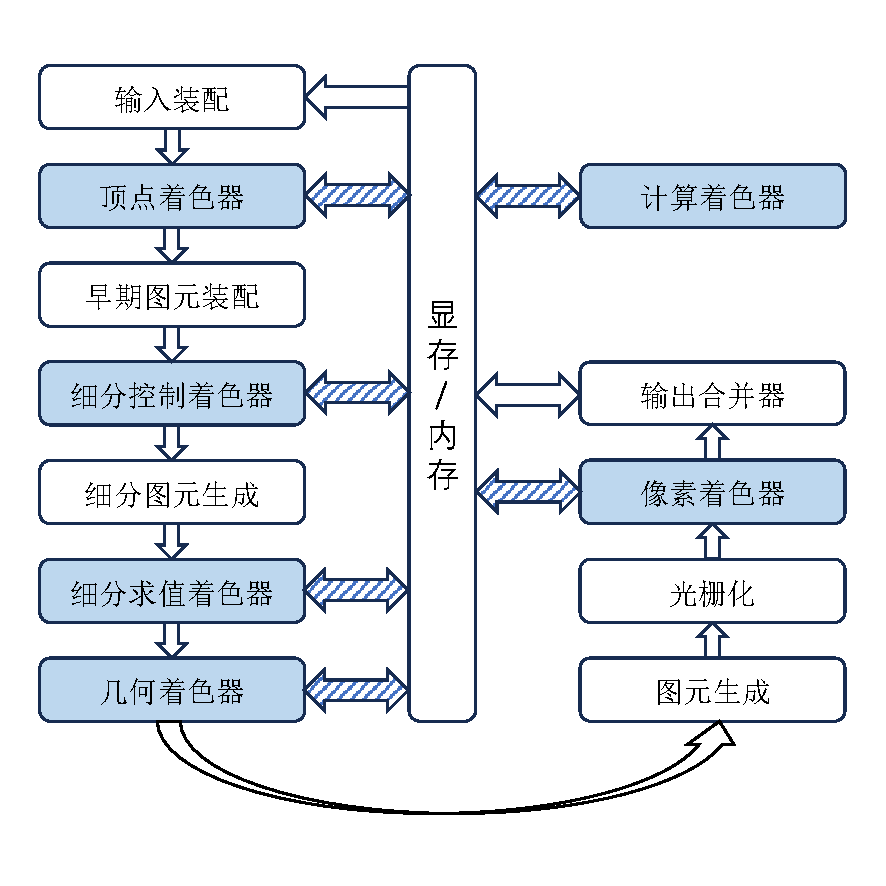
\includegraphics[page=1, width=0.7\linewidth]{figures/pictures.pdf}
    \caption{光栅化绘制流水线}
    \label{fig:rasterize_pipeline}
\end{figure}

% https://gpuopen.com/presentations/2019/nordic-game-2019-triangles-are-precious.pdf
% https://gpuopen.com/wp-content/uploads/2021/01/AMD_Graphics_pipeline_GIC2020.pdf

\begin{figure}
    \centering
    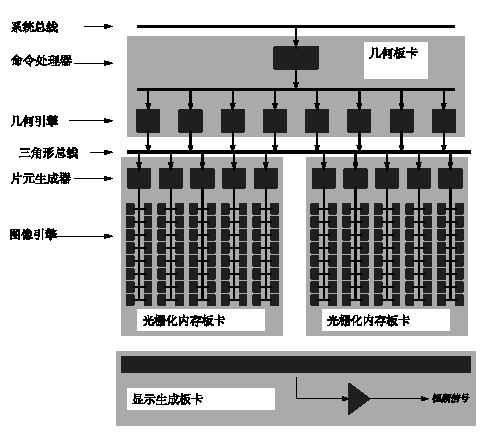
\includegraphics[width=0.8\linewidth]{figures/RealityGraphics-Page2-Crop-Zh.pdf}
    \caption{RealityEngine Graphics 架构图\cite{RealityEngineSGI}}
    \note{注:每个灰色区域代表一块独立的电路板。几何板卡为负责顶点变换的电路板,其中包含有命令处理器、几何引擎。光栅化内存板卡为光栅化电路板,其负责接收三角形,并生成对应的片元,同时进行着色操作。显示生成板卡负责连接显示器,从显存中读取图像,并负责显示信号的生成。}
    \label{fig:reality_engine_graphics}
\end{figure}

为了复用顶点着色器和片元着色器阶段中的计算单元以增加算术逻辑运算单元的利用率,从 Xbox 360 \cite{1624324}开始引入了 GPU 统一着色架构(Unified Shader Architecture),并被如 NVIDIA G80 \cite{4523358}后的 GPU 一路沿用。所谓 GPU 的统一着色架构,即包括顶点变换和屏幕空间着色等着色计算在和 GPU 共用的统一的 SIMD 处理器中进行。图 \ref{fig:volta_arch} 为 NVIDIA Volta 架构的示意图,其中包含了对于 GPU 统一计算架构来说比较关键的部分:内存、内存控制器和缓存、SM(Streaming Multiprocessor),线程块调度器和 SM 中的线程束、线程束调度器和计算功能单元。

\begin{figure}
    \centering
    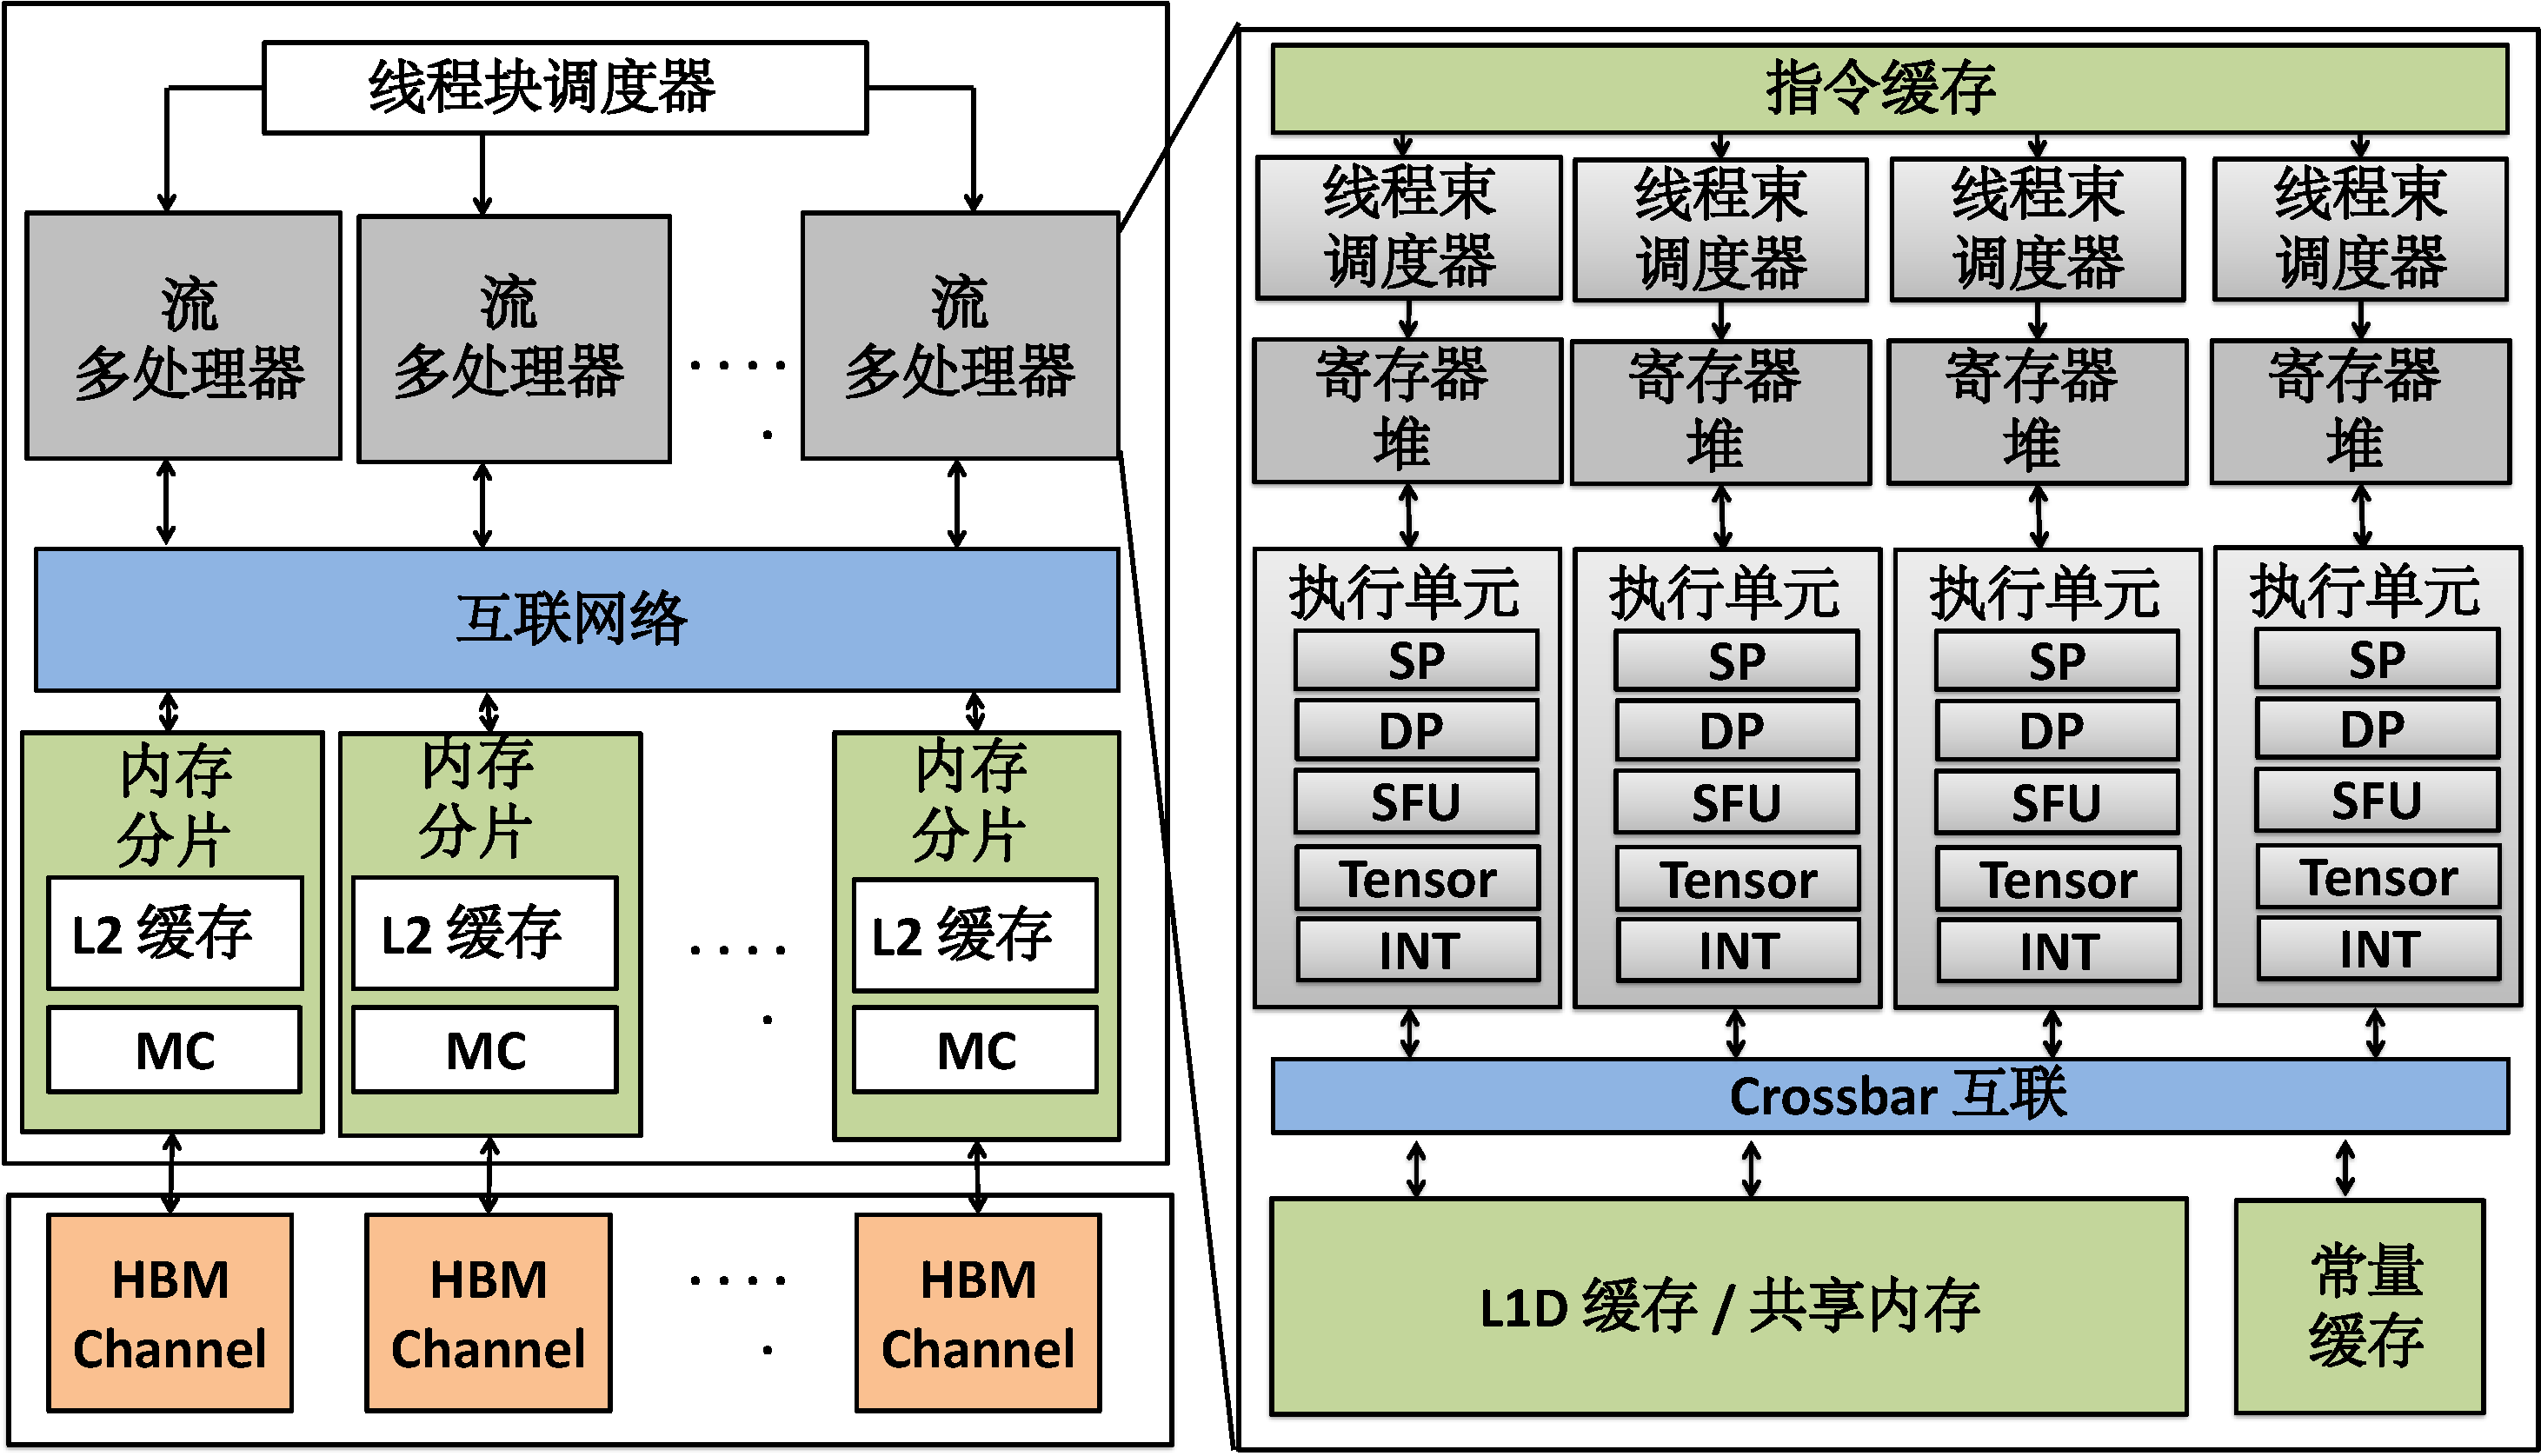
\includegraphics[width=1.0\linewidth]{figures/Volta_archi-crop-zh.pdf}
    \caption{NVIDIA Volta 架构图\cite{9138922}}
    \note{注:架构图中左边为 GPU 整体架构的示意图,由上到下分别为线程块调度器,流多处理器(SM),互联网络,内存控制器和缓存,以及对应的 HBM 内存。右侧为一个流多处理器内部的结构示意,其中由上到下分别为指令缓存、线程束调度器、寄存器堆、后端执行单元、Crossbar 互联网络、以及各个执行单元公用的共享内存和常量缓存。}
    \label{fig:volta_arch}
\end{figure}

用户在编写 CUDA、OpenCL 或者计算着色器(Compute Shader)程序时,对于 GPU 统一计算架构来说比较关键的部分概念会以较为直接的形式映射到用户编写时对应的抽象模型中。譬如,用户编写的描述单个线程行为的程序中,可以用 threadIdx(CUDA)或者 gl\_LocalInvocationID(GLSL 计算着色器)来获得当前线程在抽象的 subgroup 内的索引;再比如,用户可以使用 \_\_shared\_\_(CUDA)或者 shared(GLSL 计算着色器)来定义抽象的 subgroup 内所有线程可以访问的共享内存,这些行为会以比较直接的方式映射到计算架构上,并由具体的调度器进行调度。

然而,对于绘制流水线中的着色过程来说,上述分配则是基本不透明的。同计算着色器或 CUDA 代码一样,顶点、片元和几何着色器程序同样描述了单个“调用”所需要执行的操作;但该调用是如何映射到线程块结构来说是对用户是不透明的,且用户也无法如同计算着色器或 CUDA 核函数那样访问相邻“调用”的局部信息。事实上,这些行为多数是由设备驱动和相关的厂商的硬件实现决定的,并且和架构的实现细节密切相关。

% AMD GPUOpen
% generic informations are not available
% so, want to make step forward

部分厂商会发布面向软件开发者的较为细致的 GPU 编程指南,以供希望了解具体架构的开发者使用。Intel 周期性的发布其显示设备的参考手册,包括 Iris Xe 和 UHD 显示产品,HD 显示产品等\cite{IntelGPUManual},且其内容涵盖 GPU 中多种 IP 核的功能和编程说明、寄存器地址功能参考。AMD 则发布了其 RDNA 架构 GPU 的指令集参考手册\cite{AMDRDNAISA},其中主要描述了其 SIMD 处理器部分的指令参考。嵌入式 GPU 产品厂商也会发布其部分产品的较详细参考手册,如 Broadcom 公司发布的、用于树莓派产品的 VideoCore IV GPU 的架构参考手册\cite{V3DManual}。

然而,如果想要了解给定平台上绘制管线的硬件实现,特别是与性能相关的部分,直接通过上面的手册和材料还是相对困难的。这种困难主要来源于两个方面:其一,并非所有相关的产品细节都会有对应的文档予以发布。例如,对于性能调优有重要意义的 CUDA Binary 为闭源形式,需要进行逆向工程\cite{DecodingCUDABinary};其二,发布的文档中常常含有太多细节,以至于性能相关部分的结构和通路变得较难识别。例如,介绍 Intel Xe 和 UHD 显示核心中渲染引擎(Render Engine)的手册有 723 页,阅读这种体量的文档对于通常对细粒度的绘制流水线的硬件实现不够了解的开发者来说是一种挑战。

本研究提出的方法将着力于通过使用数据驱动的机器学习来对性能进行黑盒建模,以克服利用手册或领域知识进行逐平台的性能分析带来的时间和成本开销上的困难。

\subsection{着色器程序语言}

作为一类领域专用语言(Domain Specific Language,DSL),着色器程序语言是应用在图形 API 中,负责增强和替换图形管线中相应部分固定功能的程序和程序片段编写所用的程序设计语言。

% SEE https://www.nvidia.com/docs/IO/8227/GDC2003_OGL_ARBVertexProgram.pdf and https://www.nvidia.com/docs/IO/8228/GDC2003_OGL_ARBFragmentProgram.pdf

图形程序语言经历了一个从简单到复杂、从低级到高级的过程,这种转变趋势可以从不同的图形 API 中得到证明。2002 年,OpenGL 1.4 引入了 ARB 扩展 ARB\_vertex\_program,其中使用了较为低级的汇编指令形式来描述顶点变换阶段的用户自定义功能。在之后一年的 OpenGL 1.5 中,OpenGL 着色器程序语言 GLSL 的 1.0 版本被引入到 ARB 扩展 ARB\_vertex\_shader 和 ARB\_fragment\_shader 中,并在之后发展迭代,和 OpenGL 标准本身一起演进。

在由 Microsoft 公司主导的 DirectX 图形 API 中,也有类似的发展轨迹。2000 年的 Direct3D 8.0 中,Microsoft 公司引入了使用平台无关的汇编指令来描述顶点变换和像素着色阶段功能的着色器程序模型。之后,在 2002 年的 Direct3D 9.0 中,Microsoft 公司进一步设计了使用高级语言形式来描述顶点变换和像素着色阶段功能的高层次着色语言 HLSL(High Level Shading Language),并且在随后的标准演进中不断增加新功能。

然而,GLSL 和 HLSL 等高层次着色器程序语言因其较为丰富的语法特性,其处理和向 GPU 底层指令的转换均较为复杂。针对这类问题,Khronos Group 提出了一种统一的图形和计算 IR (Intermediate Representation,中间表示),并将其命名为 SPIR-V。经过多年的投入,SPIR-V 成为了 Vulkan 图形 API 的着色器程序输入格式,并且围绕 SPIR-V 有丰富的编译器设施。图 \ref{fig:spirv_ecosystem} 展示了这些编译设施和相应的语言概念,其中语言或指令序列以矩形展示,编译器以圆角矩形展示。

同时,从图 \ref{fig:spirv_ecosystem} 中可以看到,图形程序常用的着色器 GLSL 和 HLSL 可以分别通过 glslang 和 DXC 软件编译到 SPIR-V,进而被实现了 Vulkan 的厂商用户态驱动编译到 GPU 原生指令序列。这套链路相较 OpenGL 中将 GLSL 输入厂商用户态前端来说,因厂商间对 GLSL 语法的一些边缘情况处理不同,故而此套链路在厂商间的一致性会更好。图中的 SPIRV-Cross 软件可以实现 SPIR-V 到 GLSL 和 HLSL 的转译,与前面的前端工具配合的话,可以实现不同着色器语言的互相转换。而图中的 SPIRV-Tools 则可以实现 SPIR-V 中间表示的优化、变换、编排等操作。

% TODO introduce SPIR-V
\begin{figure}
    \centering
    \includegraphics[page=3, width=0.6\linewidth, trim=50 50 50 50, clip]{figures/pictures.pdf}
    \caption{SPIR-V 生态系统}
    % \note{注:语言或指令序列以矩形展示,编译器以圆角矩形展示。}
    \label{fig:spirv_ecosystem}
\end{figure}

本研究的主要目标为构造一个可以适用于各个平台的着色器性能预测器,这样的预测器在着色器语言方面面临着下面两方面的困难:其一,着色器程序可以以多种语言写就,如上文提到的 GLSL,HLSL,Slang,或游戏引擎等采用的更上层的中间格式,且每种格式都有一定的市场占比,没有着色器语言占有绝对的统治地位,而全部支持需要显著的开发和维护开销;其二,前面提到的高层次着色器程序语言往往拥有复杂的语法,不便于进一步的解析和处理。

故而,本研究所提出预测器基于 SPIR-V 中间表示。这样的技术选型正好可以克服上文提到的两个问题:首先,SPIR-V 拥有成熟的转译器(transpiler)生态,GLSL、HLSL 和新型的着色器程序语言 Slang 等均拥有向 SPIR-V 进行转译的工具;其次,SPIR-V 技术设计上即方便进行编译器的编写和编译变换,其采用线性 IR 指令表示,并有简洁清晰的语言规范,成熟可靠的语言优化器等,对本研究后面提及的指令追踪阶段所需要的指令编排工作有一定的帮助。

\subsection{着色器程序优化和简化}

图形 API 本身为了兼容各种不同厂商和架构的底层 GPU 硬件实现,其所希望用户程序本身呈递的着色器程序是贴近高级语言语义的、基本未经历过设备相关的优化、也没有附加很多设备相关语义的着色器程序源语言文本或中间表示。然而,出于图形程序的性能考虑,图形程序员和 GPU 设备厂商通常希望对着色器程序进行一定意义上的优化,使得其在不同或特定平台能拥有较好的实时性能。这样的要求催生了对着色器程序优化和简化的相关工作的探索。

GPU 设备厂商应用的着色器程序优化主要发生在图形程序启动时。此时,图形程序会经由图形 API 向设备驱动呈递着色器程序源码或其中间表示,此时设备驱动中的图形流水线编译器模块将会像传统的 CPU 程序编译器一样,进行源码的中间表示生成,以及编译器后端的设备无关优化、设备相关优化、寄存器分配和指令生成。在这个过程中,编译的速度和编译生成的指令序列的质量都是编译器追求的目标。即便如此,\citet{8366956} 仍然发现设备厂商的驱动并没有充分利用各种可能的着色器程序离线优化机会。\citet{8891638} 也发现,对于输入比较确定的着色器程序,仍然存在进一步优化的空间。

设备驱动中的优化需要基本保证优化后的程序符合原来输入程序的运行结果,但是对于图形应用来说,进行输出完全符合原状的着色器程序优化对于如游戏等应用场景来说并不是必需的。故而,有一系列工作 \cite{10.1145/3528233.3530722, 10.1145/2661229.2661276, 10.1145/2070781.2024186, 10.1145/2816795.2818104, 9815871} 探索了如何在有损条件下,权衡画面表现和运行性能来进行着色器程序简化。这些工作通常使用遗传算法(Genetic Programming,GP)和贪心算法来实现。在遗传算法的每步迭代中,这些工作通常会考虑各种可能对画面造成损失的简化方法:例如,将决定着色器输出的表达式的某个子表达式的值替换为零或该表达式在各种光照条件下的求解结果的平均值,或者将片段着色器阶段进行计算的值移动到顶点着色阶段等。为了进一步加快遗传算法的变异-迭代过程,\citet{10.1145/3528233.3530722} 提出了ShaderTransformer,该方法利用深度学习提出了一个着色器简化变体的渲染质量质量预测器。

\begin{figure}
    \centering
    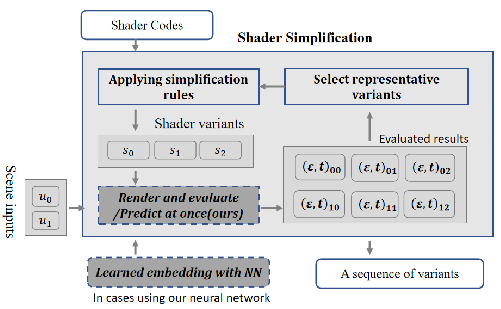
\includegraphics{figures/ShaderTransformer-Pipeline.pdf}
    \caption{ShaderTransformer 使用的着色器简化框架\cite{10.1145/3528233.3530722}}
    \label{fig:shdrTxfmr-framework}
\end{figure}

\begin{figure}
    \centering
    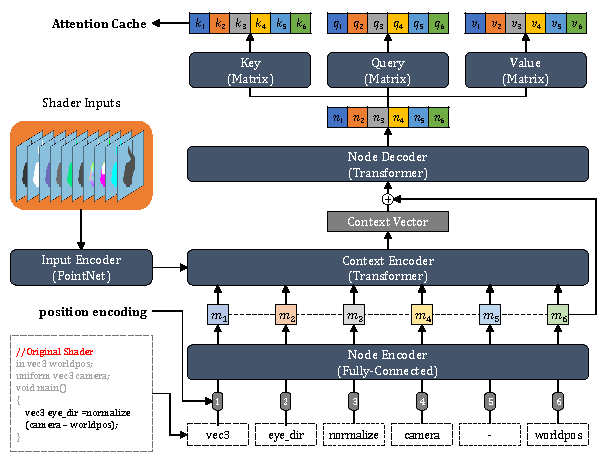
\includegraphics{figures/ShaderTransformer-Flow.pdf}
    \caption{ShaderTransformer 网络架构图\cite{10.1145/3528233.3530722}}
    \label{fig:shdrTxfmr-arch}
\end{figure}

图 \ref{fig:shdrTxfmr-framework} 给出了 \citet{10.1145/3528233.3530722} 的 ShaderTransformer 所使用的着色器程序简化框架。在每轮优化迭代中,着色器程序经过化简会形成一系列的着色器变体 $ s $,而 ShaderTransformer 可以通过 Transformer 来学习并预测每个变体在表示渲染质量中的隐空间的表示,以供评价着色器变体距离简化前的着色器的渲染质量差异 $ \epsilon $。渲染质量差异 $ \epsilon $ 和变体运行时间开销 $ t $ 会为下一步的遗传算法迭代提供参考。

值得注意的是,目前在有损着色器简化的工作通常局限于使用比较简单的启发式算法来表示着色器的运行时开销\cite{10.1145/2816795.2818104, 10.1111/cgf.13482, 10.1145/3528233.3530722},又或者每次评估变异后的着色器程序时进行单独的测量运行\cite{10.1145/2661229.2661276}。对比这些工作,本研究提出的预测器可以在不需要在目标平台上进行单独执行的条件下,对变异后着色器的运行时间开销做出更精确的预测。

图 \ref{fig:shdrTxfmr-arch} 给出了 ShaderTransformer 网络部分的架构图,其中网络的输入包括着色器程序变体的 main 入口函数的函数体源码和着色器程序变体运行时的输入,并通过编码器-解码器架构来得到在渲染质量隐空间中的特征向量。本研究也受到 ShaderTransformer 使用 Transformer 来间接预测着色器变体渲染质量的启发,同样采用 Transformer 网络来预测着色器在目标平台的性能。与其不同的是,ShaderTransformer 使用 PointNet\cite{8099499} 来提取着色器输入信息,而本研究采用了 SPIR-V 中间表示和基于 SPIR-V 的指令追踪技术,从而以统一的方式处理各种类型的输入,同时克服 ShaderTransformer 本身只能处理无分支、单函数的简单片元着色器的缺陷。

\section{程序语言理解}

\label{sec:pl_understanding}

\subsection{语言模型}

\label{sec:language_model}

语言模型是自然语言或程序语言的概率模型。一个语言模型通常定义了语言中文本 $\{l_1, l_2, ..., l_m\}$ 与分词后形成的词元 $\{w_1, ..., w_n\}$ 的对应关系,以及对于句子 $ w_1, ..., w_{i-1} $ 来说,词元 $ w_i$ 出现几率的概率模型 $P(w_i|w_{i-1}, ..., w_{1})
$。

% TODO: add bigram, trigram, ...

对于语言模型来说,将源语言文本转换为词元的分词过程对后续处理有一定影响。对于自然语言文本,各个单词出现的机率并不是均匀的,而对于出现次数过于稀疏的生僻词语,语言模型对其的概率估计总体来说较为困难。为了解决这个问题,BPE(Byte-Pair Encoding)\cite{sennrich-etal-2016-neural} 使用了一种被称为 subword 的单位来进行分词,并被 SentencePiece \cite{kudo-richardson-2018-sentencepiece} 等方法使用。

\subsection{注意力机制与 Transformer 网络}

注意力机制是模仿认知活动中注意力活动的一类神经网络机制。在使用注意力机制的网络中,通常会根据序列内容,为序列中的每个词元生成一个软的权重,并根据部分或全部序列中词元的权重来进行后续的计算。

基于 \citet{bahdanau2016neural} 中注意力机制的工作,\citet{Vaswani2017AttentionIA} 在 2017 年提出了被称为 Transformer 的神经网络结构,在自然语言处理的各类任务上均取得了巨大的成功。Transformer 网络总的结构如图 \ref{fig:transformer_overview} 所示。

\begin{figure}[h]
  \centering
  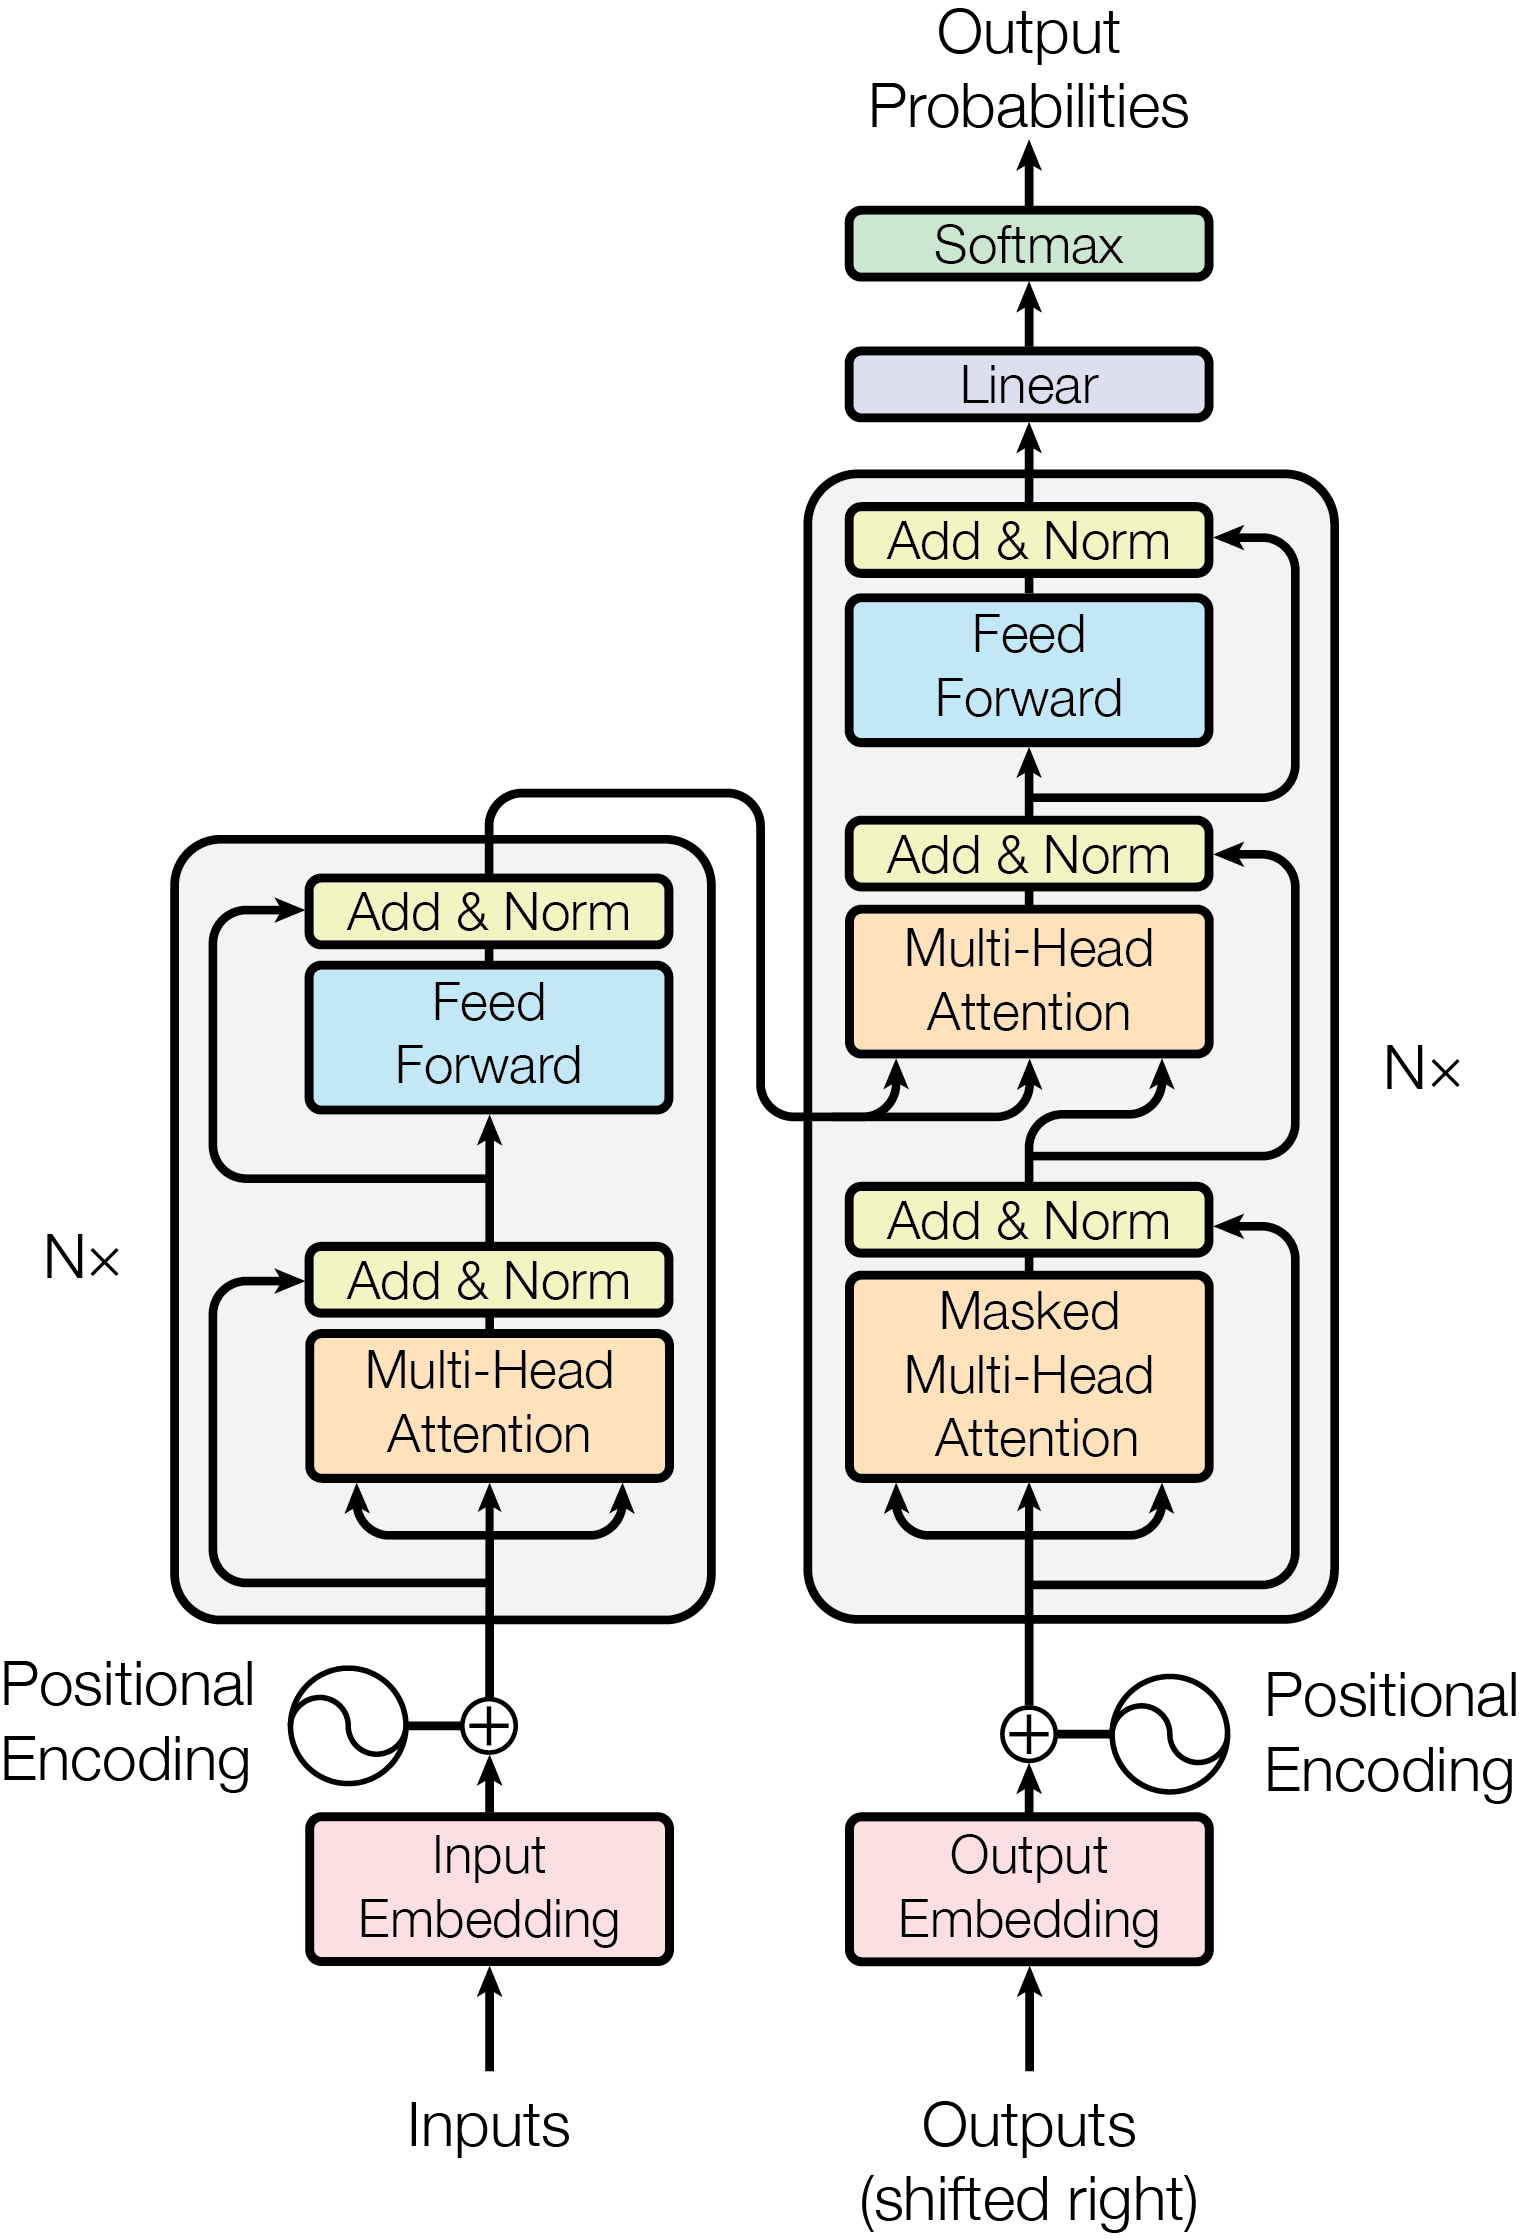
\includegraphics[width=0.5\linewidth]{figures/Transformer-Arch.png}
  \caption{Transformer 网络结构总览\cite{Vaswani2017AttentionIA}}
  % \Description{}
  \label{fig:transformer_overview}
\end{figure}

% generated by gpt3.5; TODO: rewrite

原始版本的 Transformer 模型的网络结构主要由编码器(Encoder)和解码器(Decoder)两个组件构成。Tranformer 的编码器负责将输入的序列转换为相应长度的特征向量,而 Transformer 的解码器则会利用这些特征向量来生成输出序列。

Transformer 的编码器和解码器都由多个相同的基本层堆叠而成,其每个基本层都由两个子层组成:多头自注意力层(Multi-Head Self Attention)和前馈神经网络层(Feed-Forward Neural Network)。这两个子层之间使用层归一化(Layer Normalization)和残差连接(Residual Connection)来连接在一起;同时,在层内的一些位置还会加入 Dropout 层进行归一化。

多头自注意力层由多个相同结构的自注意力层构成。在每个自注意力层中,输入的序列会被分别线性变换到三个被称为查询(Query)、键(Key)和值(Value)的序列。随后,这三个序列会进行一个被称为缩放点积注意力(Scaled dot product attention)的操作
$$
\operatorname{Attention}(Q, K, V) = \operatorname{softmax}\left(\frac{Q K^T}{\sqrt{d_k}}\right)V,
$$
其中 $Q$ 为查询,$K$ 为键,$V$ 为值,$d_k$ 为键的维度。

这种类型的注意力机制可以允许序列中任意的两个位置的词元交换信息,且通过注意力分数来表征了每个位置对其他位置的“重要性”,从而实现了序列中不同位置之间的交互和信息传递。

将维数为词元嵌入维度 $ d_{model} $ 的序列并行的进行多组自注意力操作可以改善模型表现。多个这样的注意力机制进行拼接的结果为多头注意力,其计算方式如下:
$$
\operatorname{MultiHead}(Q, K, V) = \operatorname{Concat}(head_1, ..., head_h) W^{O}
$$
其中 $head_i$ 为第 $ i $ 组独立的进行自注意力计算的计算结果。

多头自注意力层之后,连接的另一个重要模块是前馈神经网络层。该层由两个全连接层组成,并通过 ReLU 函数进行激活,其计算方式如下:
$$
\operatorname{FFN}(x)= \max(0, x W_1 + b_1) W_2 + b_2
$$

原始的 Transformer 中同时使用了编码器和解码器,而编码器和解码器之间还有一个重要的结构:编码器-解码器注意力层(Encoder-Decoder Attention)。在解码器中,每个位置的输出依赖于编码器中所有位置的输入。为了实现这种全局的依赖关系,解码器的多头注意力层中使用了编码器的输出来作为查询 $Q$ 和键 $K$。

总体来看,Transformer 模型通过自注意力机制和多头注意力机制,有效地捕捉了输入序列中的全局依赖关系,并在许多自然语言处理任务中取得了显著的性能提升。例如,BERT \cite{devlin-etal-2019-bert} 模型就利用预训练的范式,在 Transformer 编码器的基础上利用掩码语言建模(Masked Language Modeling)和后续语句预测(Next Sentence Prediction)任务在大规模预料上进行预训练,其在下游任务上只需接受较少的微调即可达到较好的性能。

\subsection{程序设计语言理解任务}

程序设计语言可以被看作一种特殊形式的语言,故而很多自然语言处理领域的方法也适用于程序设计语言的相关任务中。在如 Transformer\cite{Vaswani2017AttentionIA} 和 BERT\cite{devlin-etal-2019-bert} 等模型的影响下,业界涌现出了一批用于程序设计语言任务的模型,如 CodeBERT\cite{feng-etal-2020-codebert},GraphCodeBERT\cite{DBLP:conf/iclr/GuoRLFT0ZDSFTDC21} 等。

\begin{figure}
    \centering
    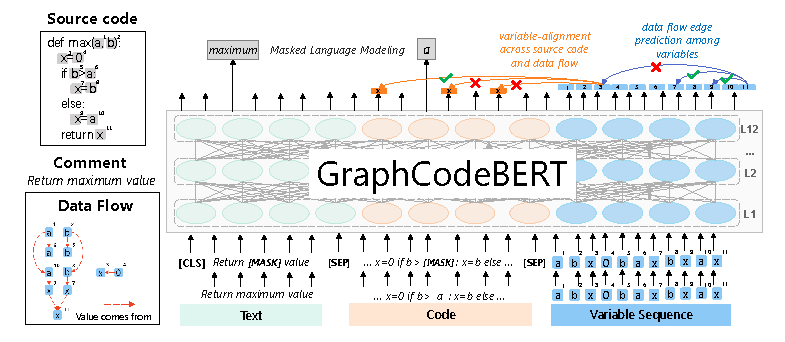
\includegraphics[width=1.0\linewidth]{figures/GraphCodeBERT-Crop.pdf}
    \caption{GraphCodeBERT 架构和预训练示意图\cite{DBLP:conf/iclr/GuoRLFT0ZDSFTDC21}}
    \label{fig:graphCodeBERT_arch_and_pretrain}
\end{figure}

以 GraphCodeBERT 为例,图 \ref{fig:graphCodeBERT_arch_and_pretrain} 给出了 GraphCodeBERT 的架构以及其预训练任务示意图。在模型的训练阶段中,GraphCodeBERT 模型使用了带有注释的源代码和其对应的数据流信息作为输入,并用掩码语言建模和两个和程序语言理解相关的结构化任务来进行预训练。这两个结构化任务分别要预测数据流中的边的起点和终点、以及数据流节点和代码中变量的对应关系。通过模型在大规模程序语料上的预训练工作,特别是程序相关的数据流任务的预训练工作,模型可以提升对于程序设计语言的理解能力,进而提升在如代码搜索、克隆检测等下游任务上的性能表现。

GraphCodeBERT {\amend 的工作同时说明},代码的中间表示形式(如抽象语法树)相比源代码文本,能提供更丰富的结构化信息。故而,本研究选择首先将着色器程序编译为中间表示,以作为模型的输入。同时,GraphCodeBERT 等模型采用 Transformer 来程序的变量和指令之间的上下文依赖关系,类似的,本研究的工作也采用 Transformer 来捕捉着色器指令间的上下文相关性,来将更多的上下文信息引入到性能建模中。

根据 \citet{ijcai2022p775} 的综述,程序语言理解模型的典型应用包括抄袭检测,代码分类,代码缺陷检测,代码翻译,代码检索等。同时,也存在被设计为捕捉性能相关的语义的一类任务,譬如在 \citet{8091247} 的工作中引入,并被后续工作 \cite{pmlr-v139-peng21b, pmlr-v139-cummins21a} 用于评价模型质量的 OpenCL 异构架构映射任务。该类任务的输入是一系列 OpenCL 核函数(kernel function),程序语言理解模型需要给出某个具体的核函数在何种平台上运行较快的分类值。笔者希望,通过本研究过程中收集的着色器性能数据,可以启发出更多关于程序语言模型中进行性能语义理解任务的工作。

\section{程序性能建模}

程序性能建模对于计算机软件架构设计和实现中的众多决策都有比较重大的意义,所以学术界开展了大量的、不同计算平台上的,对在 CPU,GPU 和其它加速器上运行的程序进行程序性能估计的工作。这些工作可以依照其建模方法大致分为两种类型的模型:\textbf{基于分析的模型}和\textbf{基于学习的模型}。同时,本章还简要介绍了对于 GPU 上图形系统建模的相关工作。

% Performance modeling is crucial for many design decisions; consequently, extensive research has been dedicated to the estimation of program performance on various computing platforms, including CPU, GPGPU, and other Domain-Specific Architectures (DSAs). Predominantly, the field employs two categories of models: analytical-based models and learning-based models. Works on graphics performance modeling are also discussed in this section. 

\subsection{基于分析的模型}

基于分析的模型可以大致分为\textbf{体系结构模拟器}和\textbf{简单分析模型}两类。

体系结构模拟器是针对性能关键部件进行建模以达到在时钟周期数量级上精确的,人工编写的模拟器。比如,NaviSim \cite{10.1145/3559009.3569666} 是为 AMD RDNA 通用 GPU 架构设计的模拟器,其通过为 wavefront 调度,RDNA 指令发射、解码和执行阶段编写模拟例程来实现计算核函数性能的预测。GPGPU-Sim \cite{9138922, 4919648} 是面向在 NVIDIA GPU 上执行的 CUDA / OpenCL 算例编写的模拟器。

简单分析模型是利用简单的抽象来捕捉其预期描述的架构的公共部分的一类分析模型。这类模型中比较主流的模型有 Roofline 模型\cite{10.1145/1498765.1498785, KONSTANTINIDIS201737}和流水线模型\cite{LEMEIRE202332, 10289219, 10.1145/3524059.3532396}。 

以 Roofline 模型为例,该类模型主要通过利用计算系统中存储器和运算器两个方面的基础数据,来给出待建模系统在稳态条件下的峰值性能估计。

具体来说,Roofline 模型用如下参数刻画给定应用或算例的基本性质:

\begin{itemize}
    \item $W$: 对于给定应用或算例的总计算数目,单位为 FLOP (浮点运算数, FLoating point OPerations)
    \item $Q$: 对于给定应用或算例的总内存访问数,单位为字节
    \item $I = W/Q$: (\textbf{计算强度}, Arithmetic Intensity) 单位内存访问可以完成的计算数目,单位 FLOP/字节
\end{itemize}

此外,定义

\begin{itemize}
    \item $\pi$: 峰值性能,单位为 FLOPS (每秒浮点运算数, FLoating OPeartions per Second)
    \item $\beta$: 峰值存储器带宽,单位为 字节/秒
\end{itemize}

Roofline 模型定义的给定程序的\textbf{可达性能} P 则可以由下式计算:
$$
P = \min(\pi, \beta \cdot I)
$$

从而,可达性能 $ P $ 关于计算强度 $ I $ 的关系又可以用图 \ref{fig:roofline_graph} 来表示。图中曲线即为应用程序在该平台上应用 Roofline 模型计算出来的理论性能峰值,可以看到随着应用程序本身的性质带来的计算强度 $ I $ 的改变,其可达性能可以拥有不同的值。图 \ref{fig:roofline_graph} 中的 I 区域代表由于内存带宽限制了可达性能的访存瓶颈(Memory bound)区,而 II 区域代表由于运算器速率限制了可达性能的计算瓶颈(Compute bound)区。这里假设计算系统参数 $\pi$ = 10 FLOPS,$\beta$ = 1 字节。

值得注意的是,由于指令并行度、发射冲突等架构设计原因,即使理论的内存带宽充足,应用程序对应的指令序列仍可能在使用运算器时遇到无法达到理论的运算器使用率的情形,此时应用程序的性能将低于 Roofline 模型给出的可达性能。同时,由于各种图形处理器中存储器层次结构的存在,不同的存储器层次拥有不同的总带宽,此时有效带宽也将和具体的程序发生耦合,让此类模型的预测变得更加困难。

\begin{figure}[h]
  \centering
  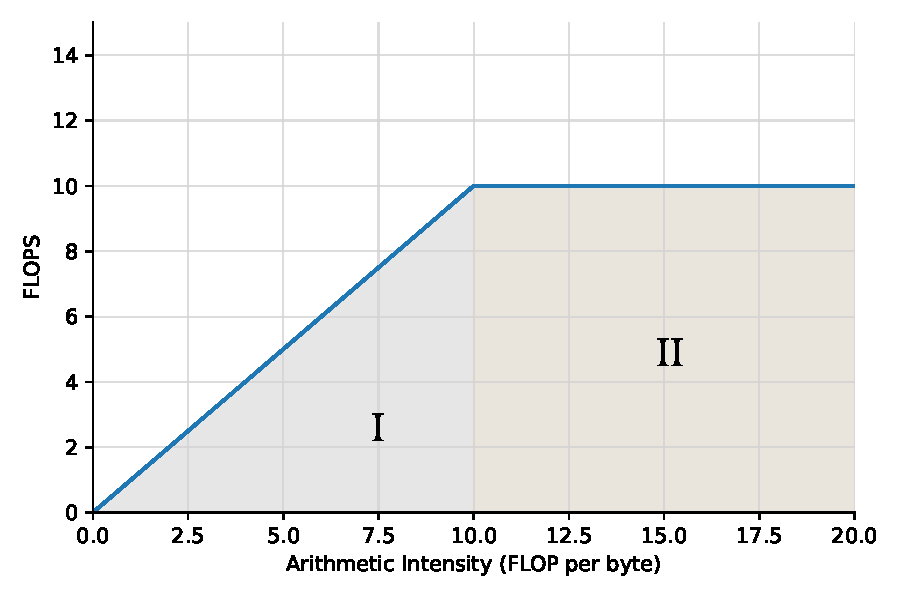
\includegraphics[width=0.7\linewidth]{figures/roofline.pdf}
  \caption{Roofline 模型中可达性能 $ P $ 关于计算强度 $ I $ 的关系图}
  % \note{注:图中的 I 区域代表由于内存带宽限制了可达性能的访存瓶颈(Memory bound)区,而 II 区域代表由于运算器速率限制了可达性能的计算瓶颈(Compute bound)区。这里假设计算系统参数 $\pi$ = 10 FLOPS,$\beta$ = 1 字节。}
  \label{fig:roofline_graph}
\end{figure}

总的来看,基于分析的模型的优秀表现依赖于对待建模架构的深入理解,以及对待建模架构的较详细的微架构基准测试。这赋予了这类模型相对精确的精度,然而也让此类模型的通用性下降。故而,本文提出的方法选择使用基于学习的模型。

% Analytical-based models can be roughly divided into \textit{architecture simulators} and \textit{simple analytical models}. \textit{Architecture simulators} are hand-crafted simulators that are usually cycle accurate for the architecture components that are related to performance. For example, NaviSim \cite{10.1145/3559009.3569666} is a simulator for AMD RDNA architecture, giving predictions on compute kernel execution time by writing simulation procedures for wavefront dispatching, RDNA instruction issuing, decoding and execution. GPGPU-Sim \cite{9138922, 4919648} is a simulator for CUDA / OpenCL workloads that runs on NVIDIA GPUs. \textit{Simple analytical models}, on the other hand, tend to use simple abstractions that capture the common aspects for the architecture family they model. Popular choices of these models includes the roofline model \cite{10.1145/1498765.1498785, KONSTANTINIDIS201737} and the pipeline model \cite{LEMEIRE202332, 10289219, 10.1145/3524059.3532396}. To summarize, analytical-based models in general require a in-depth understanding of the architecture they model as well as extensive micro-benchmarks related to characteristics they capture.

\subsection{基于学习的模型}

% Learning-based models alleviate the need for detailed architecture inspection by using machine learning, and they are much easier to be ported to new architectures given measurements on new architectures. Several works estimate basic block throughput on CPU using either hierarchical LSTM \cite{pmlr-v97-mendis19a} or Graph Neural Network (GNN) \cite{9975403} capturing from in-the-wild application profiles \cite{pmlr-v97-mendis19a, 9042166}. \citet{10.1145/3575693.3575737} modeled the tensor program tuning problem as a Natural Language Processing (NLP) regression task.

相比于基于分析的模型,基于学习的模型通过机器学习的办法,从目标架构的测量数据出发来以较为统一和自动的方式进行架构性能的建模。例如,一些工作采用层次化 LSTM 网络或 GNN 网络 \cite{pmlr-v97-mendis19a, 9975403}来预测给定中央处理器上的基本块吞吐率。如 \citet{10.1145/3575693.3575737} 的工作则将张量程序调优的问题建模为一个采用自然语言处理领域技术的回归任务。

一个比较典型的例子是 Ithemal \cite{pmlr-v97-mendis19a}。如图 \ref{fig:ithemal_overall} 所示,该工作利用了一个 Hierarchical LSTM 网络来预测一个基本块的吞吐率。每条基本块中的指令会经历一个正则化过程来将源操作数、目标操作数等处理成为统一的形式,并送入指令层 LSTM 中。随后,每个指令的隐藏层表示会被送入预测层,并在输入整个序列后输出对该基本块在给定平台上吞吐率的预测。

\begin{figure}[ht]
  \centering
  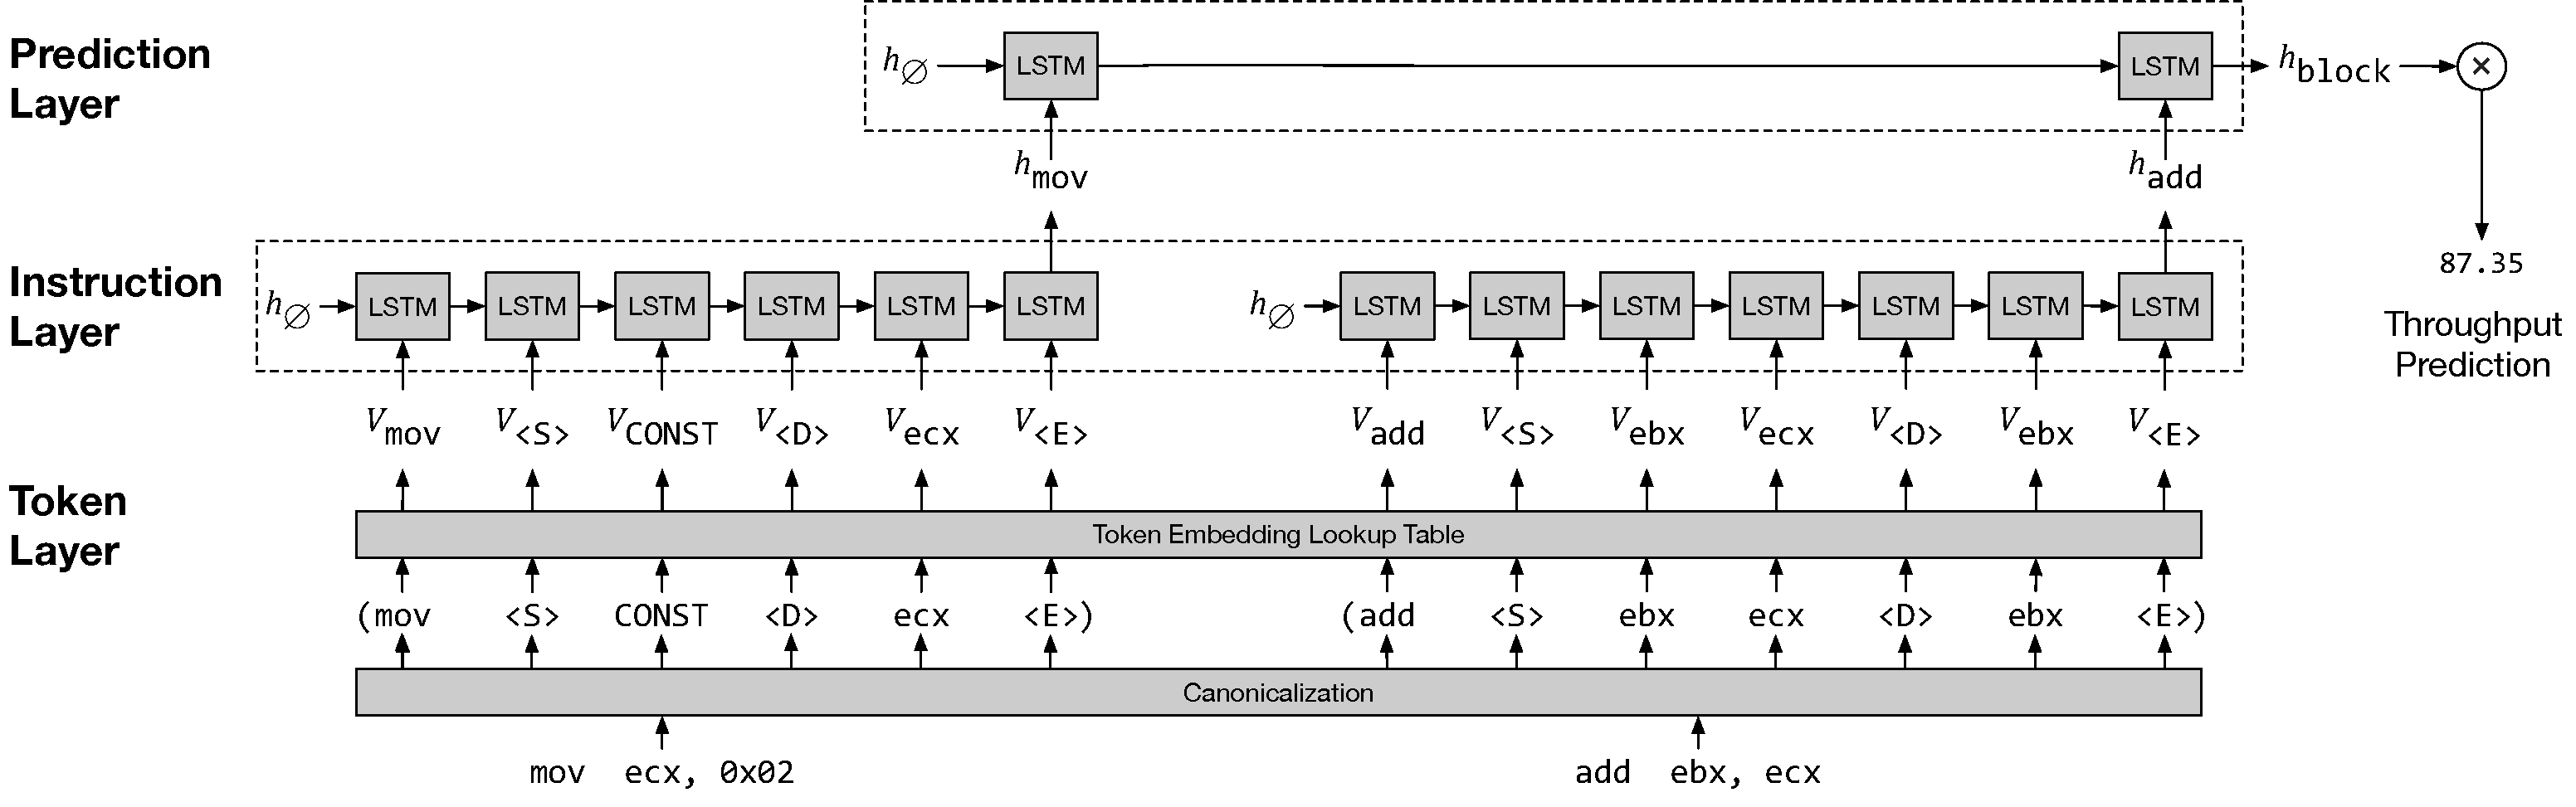
\includegraphics[width=\textwidth]{figures/diag_fullsystem.pdf}
  \vspace{-20pt}
  \caption{Ithemal 网络结构\cite{pmlr-v97-mendis19a}}
  \label{fig:ithemal_overall}
\end{figure}

对于基于学习的模型来说,一个全面而有代表性的训练数据集是模型质量的重要组成部分。Ithemal 的数据集来源于有代表性的用户和系统软件的二进制程序文件,并利用 Dynamorio \cite{10.1145/2365864.2151043} 来导出基本块数据。

% A portion of performance models focus on modeling graphics system performance. \citet{10.1145/3126557} have built a predictive model using random forests for GPU graphics workloads targeting on Intel Skylake integrated graphics, using the internal cycle-accurate simulator as target for alignment. \citet{10.1145/3307650.3322221} proposes Emarald, a SoC simulator built upon GPGPU-Sim \cite{4919648} for graphics and GPGPU system modeling. \citet{8167756} builds GLTraceSim, a framework for generating and replaying CPU and GPU memory traces under graphics workload.

% Our work proposes a learning-based model, as GPU tends to have big architecture differences across vendors and generations. To our knowledge, there are currently no publicly available cross-vendor GPU performance models that focus on shader performance modeling and operate in a black-box fashion, and this work aims to bridge this gap.

本文提出的着色器程序性能预测模型属于基于学习的模型,因为 GPU 架构在不同厂商和产品线间通常差异较大,而基于学习的模型会较易迁移。据作者所知,目前尚不存在面向着色器程序、适用于不同厂商的黑盒性能模型,而本文提出的方法将致力于填补这一空白。类似 Ithemal,本文也收集了自己的性能数据集,以服务后续的性能预测模型的学习。

\subsection{图形系统建模}

% TODO: expand each of the following into a paragraph

一部分性能模型专注于图形系统性能的建模。本节将简要总结这些模型和提出这些模型的工作。

针对 Intel Skylake GT3 显示核心,\citet{10.1145/3126557} 构建了一个预测模型来预测给定图形负载设定下每帧绘制完成所需的的时钟周期数(Cycle Per Frame,CPF)。该预测模型采用随机森林来回归利用截帧工具截取的、来自不同游戏的 Direct3D 视角下的一帧,并且其输入是软光栅器渲染该帧时的一些绘制流水线统计数据。该方法本质上是为加速厂商内部使用的硅前性能验证工具服务的,因为其预测输出的回归目标是 Intel 内部使用的专有硅前仿真软件 GPUSim 输出的该帧时钟周期数值,且利用随机森林和软光栅器的方案相较于该时钟精确的 GPUSim 软件来说可以达到平均 327 倍的加速。

\citet{8167756} 提出了 GLTraceSim,一个用于分析 GPU 平台下 GPU 和 CPU 内存系统通信的框架。该框架主要包括截帧、生成内存追踪信息、重放内存追踪信息和分析四个步骤。和 \citet{10.1145/3126557} 的工作类似,该工作也是通过软光栅器来提取相应的传输特征,并且送入相关的细粒度模拟器进行模拟的。图 \ref{fig:gltracesim} 给出了GLTraceSim 中内存访问和 CPU/GPU 同步模拟的大致流程。可以看到,相比于\citet{10.1145/3126557}的工作,GLTraceSim 更详细的抽出了软光栅器 LLVMPipe 中可能与 CPU/GPU 内存访问和同步的相关信息,并且在一个内存系统模拟器上重放来评估给定架构下内存系统的工作效率。

\begin{figure}
    \centering
    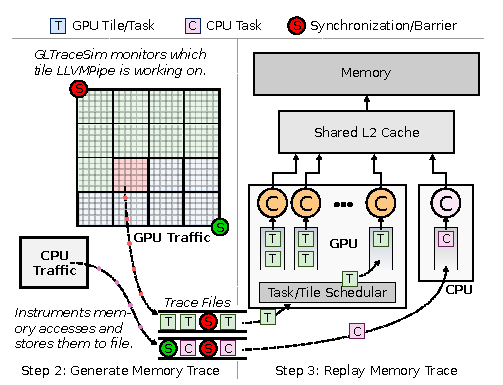
\includegraphics{figures/GLTraceSim.pdf}
    \caption{GLTraceSim 中内存访问和 CPU/GPU 同步模拟流程图\cite{8167756}}
    \label{fig:gltracesim}
\end{figure}

% https://zhuanlan.zhihu.com/p/615066252 - replacement for \textcircled

不过,以上两类工作都只是对 GPU 绘制过程中的部分模块进行了仿真,并提出一些性能特征因子以供下游预测或模拟使用。\citet{10.1145/3307650.3322221} 则更进一步,提出了全系统模拟的 Emarald,一个基于GPGPU-Sim \cite{4919648} 的、可以建模整个 SoC 的内存和计算行为的模拟器。该模拟器可以支持 OpenGL 和 OpenGL ES 着色器的模拟,同时可以配合 gem5 一起进行 Android 全系统模拟。

如图 \ref{fig:emerald_gpu_arch} 所示,Emerald 仿真中的 GPU 包括一个共享的、支持原子操作的 L2 缓存和一系列 SIMT Cluster,其中每个 SIMT Cluster 中的结构如图 \ref{fig:emerald_units}(a) 所示。在每个 SIMT Cluster 中,包括 \ding{172} 中的 SIMT 核心以及 \ding{173} 到 \ding{179} 表示的固定管线单元。渲染管线的顶点着色阶段会在 \ding{172} 中的 SIMT 核心中运行顶点着色器,并由 SIMT 核心将生成后的顶点位置信息送到顶点处理和运算单元 VPO 中。

VPO 的结构如图 \ref{fig:emerald_units}(b) 所示,其会将变换后的图元按屏幕空间的特定顺序分配给不同的 SIMT Cluster。为了实现这个目的,VPO 会将送入的顶点束(vertex warp)进行顶点对应的图元的包围盒计算,并给出其在每个 SIMT Cluster 中是否存在的掩码,之后通过互联网络进行重排序,以让每个 SIMT Cluster 的光栅器最后处理本 SIMT Cluster 负责的屏幕空间区域的图元的光栅化操作。

\begin{figure}
    \centering
    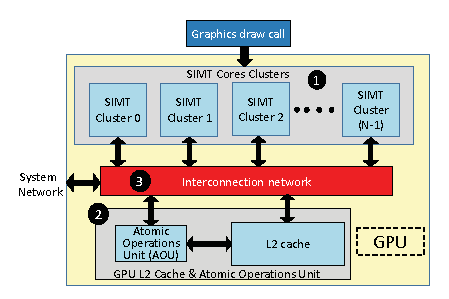
\includegraphics{figures/emerald_gpu_arch.pdf}
    \caption{Emerald 中仿真的 GPU 架构示意图\cite{10.1145/3307650.3322221}}
    \label{fig:emerald_gpu_arch}
\end{figure}

\begin{figure}
    \centering
    \begin{minipage}[b]{\textwidth}
        \begin{subfigure}[b]{0.48\textwidth}
            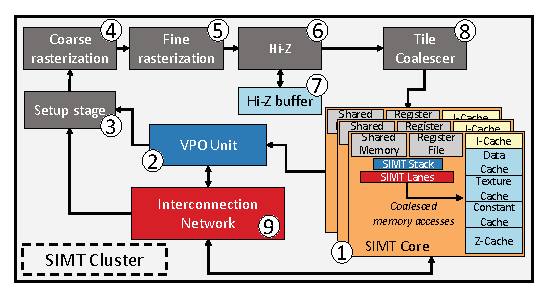
\includegraphics[width=\textwidth, trim=5 0 0 0, clip]{figures/emerald_simt_cluster.pdf}
            \caption{Emerald 中仿真的 SIMT Cluster 示意图}
            \label{fig:sub_simt}
        \end{subfigure}
        % \hfill % Adds horizontal space between the subfigures
        \begin{subfigure}[b]{0.48\textwidth}
            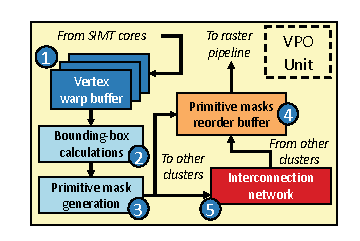
\includegraphics[width=\textwidth, trim=0 5 0 0]{figures/emerald_vpo_unit.pdf}
            \caption{Emerald 中仿真的 VPO 单元示意图}
            \label{fig:sub_vpo}
        \end{subfigure}
    \end{minipage}
    
    %\vspace{1em} % Adds vertical space between the rows of subfigures

    % TODO: add reference
    \caption{Emerald 中仿真的 GPU 架构中的细粒度单元示意图\cite{10.1145/3307650.3322221}}
    \label{fig:emerald_units}
\end{figure}

% TODO: crop the picture and explain; SC is shader core, inside which it does the detailed emulation, so no magic here



% TODO: summarize

总的来说,这些工作多着眼于和给定的图形处理器架构精确对齐,且大多需要对待建模架构的较深入理解,或者一些厂商内部模型的指导。故而,其对于图形程序员的帮助有限,且测试和使用均需要逐平台进行,因而也受到跨平台性能调优面临的平台碎片化的困难的影响。正因如此,本研究选择从数据驱动驱动的方法出发,通过神经网络方法来建模着色器程序的性能。


\section{{\added 本章小结}}

{\added 本章主要介绍了着色器性能数据集和着色器性能预测工作的相关工作和基础知识。本章介绍了 GPU 上的实时渲染和着色器程序语言,Transformer 和语言模型的基础知识,随后回顾了着色器程序优化、程序语言理解和程序性能建模三个方面的工作,并针对每个三方面中每种类型的工作,探讨了其优势和劣势。}
\chapter{基于神经网络的着色器程序性能预测方法}

\section{方法总览}

\begin{figure}[h]
  \centering
  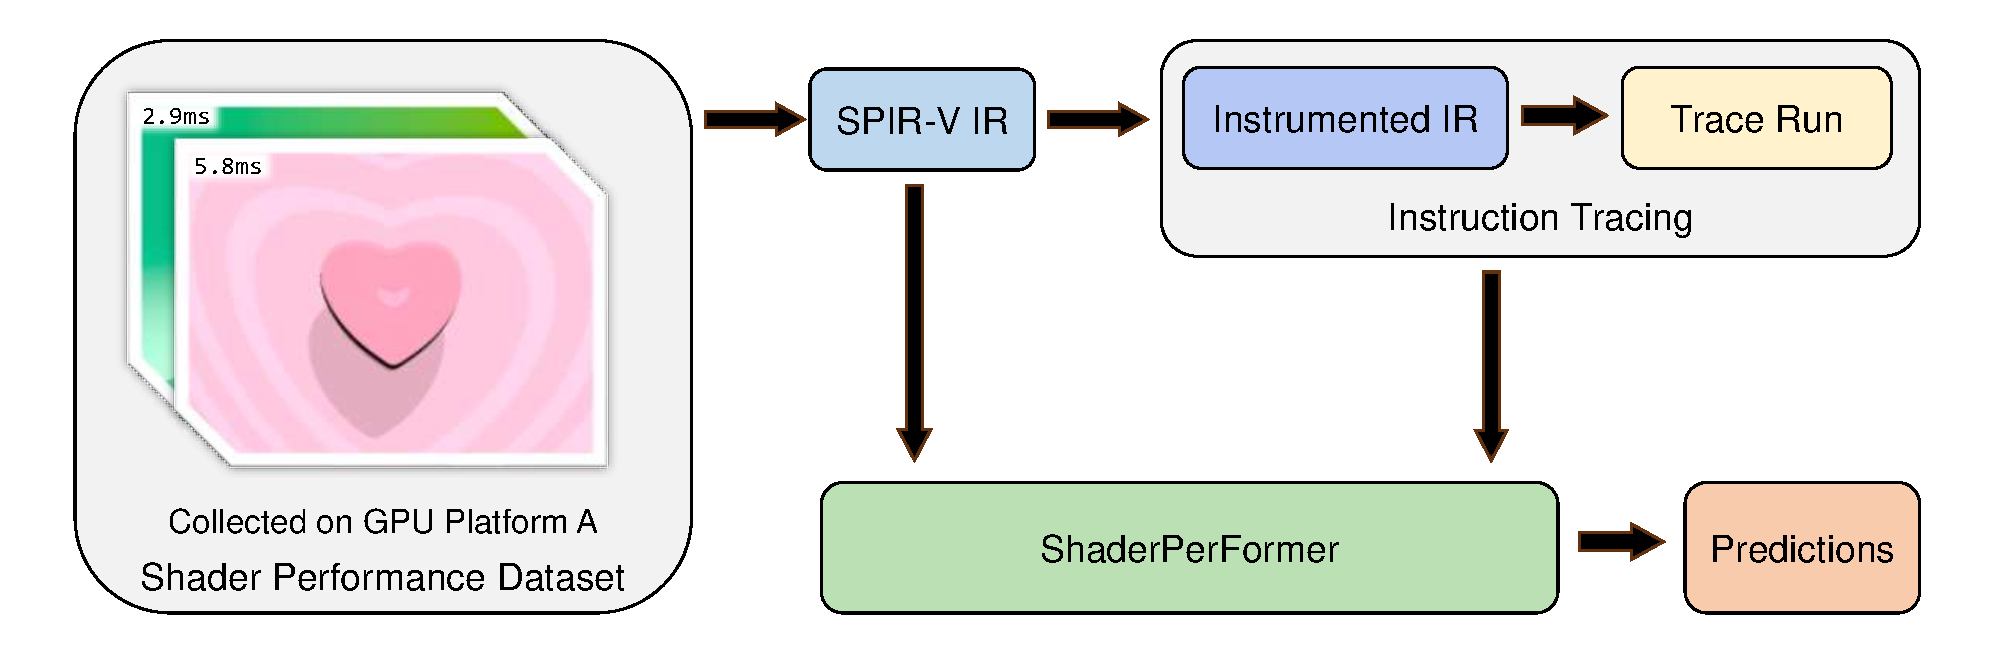
\includegraphics[width=1\linewidth]{figures/OverviewNewNewNew.pdf}
  \caption{本文提出的方法总览。 GPU 平台 A 是待建模的 GPU 平台,本文提出的模型使用 GPU 平台 A 上收集到的性能数据进行训练。}
  % \Description{}
  \label{fig:pipeline_overview}
\end{figure}

% generated by kimi.ai

本研究提出的方法构建了一个针对特定图形处理平台的着色器性能预测模型。该方法可以分为几个主要步骤:着色器数据集构造,着色器指令追踪,以及利用模型进行性能预测。这些环节的大致流程如图 \ref{fig:pipeline_overview} 所示。

首先,为了预测目标图形处理器平台的着色器性能,本方法需要收集一个详尽的着色器性能数据集,该数据集收集过程的具体讨论可以参见第 \ref{sec:dataset} 节。该数据集不仅包含丰富的着色器 GLSL 源代码、编译后的 SPIR-V 中间表示,还包括每次着色器在目标平台运行时着色器的 Uniform 输入参数,以及这些着色器在目标 GPU 平台运行测得的执行时间。这些数据是本方法所述预测器学习理解着色器性能的“原材料”,也为后续的模型训练和验证提供了比较扎实的基础。

数据收集完成后,本文提出的方法的下一个任务是,构建一个基于学习的、能够准确预测着色器在目标 GPU 平台上执行时间的模型。为了达成这个目标,该模型使用两类输入:一是以 SPIR-V 中间表示格式来进行表示的着色器指令;二是与该着色器的指令执行跟踪信息。

原始指令的收集,是通过使用业界标准的着色器编译器 glslang \cite{glslang} 实现的,而着色器执行跟踪信息则是通过一个专门的指令跟踪阶段(见第 \ref{sec:tracing} 节)来获取的。在指令跟踪阶段,本方法提出的过程会对着色器原始的 SPIR-V 中间表示插入额外的跟踪指令,然后运行修改后的中间表示,来统计出执行过程中 SPIR-V 粒度的指令运行计数。这些带有跟踪指令的 SPIR-V 中间表示可以在目标平台运行,也可以在其它非目标平台运行。通过着色器指令跟踪过程,本方法能够较为准确地追踪和分析着色器的执行行为,而无需再在目标平台上实际的执行着色器程序。

随后,本方法将收集到的 SPIR-V 指令和着色器执行跟踪信息一同,输入到构建的神经网络模型 (见第 \ref{sec:model})中。该模型将根据这些输入进行推理,得到对绘制一帧所需的时间的预测。我们利用数据集中的测量的真实值来构造损失函数,从而对模型进行优化。

% generation end

\section{着色器程序性能数据集}

\label{sec:dataset}

% generated by kimi.ai

为了学习着色器程序的性能,我们首先需要丰富的着色器程序。针对这一点,本方法选择利用 Shadertoy \cite{Shadertoy} 平台上用户上传的着色器资源。

Shadertoy 是一个在线平台,它允许用户创建、分享和查看着色器程序及其实现的效果。Shadertoy 平台上的着色器通常假设在顶点阶段处理一个四边形,而所有核心逻辑都在片元阶段执行。这为深入研究片元着色器的性能提供了相对有利的条件。

尽管在渲染时缺乏多样的几何输入,在 Shadertoy 上进行开发的用户仍然可以通过应用如 Ray Marching \cite{Hart1996}, 过程化内容生成 (Procedural Content Generation) 等技术来创建能够产生复杂视觉效果的着色器。图 \ref{fig:shadertoy_gallery} 展示了一些 Shadertoy 中着色器使用的技术和使用的技术路线。

\begin{figure}[htbp]
     \centering
     \begin{subfigure}[b]{300}
         \centering
         
\includegraphics[width=\textwidth]{figures/shadertoy_cloud.png}
         \caption{$y=x$}
         \label{fig:y equals x}
     \end{subfigure}
     \hfill
     \begin{subfigure}[b]{300}
         \centering
         
\includegraphics[width=\textwidth]{figures/shadertoy_cloud.png}
         \caption{$y=3\sin x$}
         \label{fig:three sin x}
     \end{subfigure}
        \caption{Three simple graphs}
        \label{fig:three graphs}
\end{figure}


这些着色器的性能表现在相关文献 \cite{https://doi.org/10.1111/cgf.14457} 中有所探讨。因此,本方法认为Shadertoy上的着色器在片元着色器性能建模方面具有代表性。

\paragraph{收集}
本方法通过Shadertoy网站提供的API接口,收集了27911个着色器。

\paragraph{编译}
从Shadertoy下载的着色器包含一个名为 \verb|mainImage| 的入口函数。本方法将 \verb|mainImage| 封装为片元着色器的入口点,并在统一块中引入如 \verb|iTime| 和 \verb|iResolution| 等 Uniform 变量。随后,使用glslang编译器将这些着色器编译为SPIR-V中间表示。

\paragraph{性能分析}
本方法开发了一个名为 \verb|vkExecute| 的Python扩展来测量着色器的性能。核心的性能分析逻辑在算法~\ref{alg:profile} 中详细描述。为了减少CPU提交的开销,本方法采用基于GPU的时间戳计数器来精确测量执行时间。\verb|unitTs| 表示计数器每次增加所对应的时间间隔,这一值依赖于具体的硬件平台。为了进一步降低GPU绘制的开销,本方法在时间戳计数器读取之间额外发出 \verb|num_cycles| 次绘制命令(见概念\label{concept:numCycles}),因为许多收集到的着色器在现代 GPU 平台上的执行速度非常快(>1000fps)。此外,为了确保结果的准确性,本方法进行了 \verb|num_trials| 次 GPU 命令提交(见概念\label{concept:numTrials}),并将所有测量结果存储以供后续分析。在所有性能分析过程中,本方法通过供应商提供的接口锁定了测试平台上的着色器和内存时钟频率。

\paragraph{错误恢复}
Shadertoy平台并不对用户提交的着色器进行合法性验证,因此编译错误在所难免。同时,由于着色器已经成为图灵完备的领域特定语言(DSL),其执行时间可能没有上限,这可能导致现代 GPU 驱动程序在渲染命令耗时过长时触发引擎或 GPU 的重置。当此类重置事件发生时,分析器的 Vulkan 上下文可能会失效。为了避免管理程序被意外终止,本方法将着色器性能分析任务分散到多个独立进程中进行。

% generate end

\begin{algorithm}
\caption{性能分析例程伪代码}
\label{alg:profile}

\SetAlgoLined % For setting line numbering
\SetKwFunction{FProfileShaderOnce}{ProfileShaderOnce}
\SetKwFunction{FProfileShader}{ProfileShader}
\SetKwProg{Fn}{Function}{:}{}
\SetKwInOut{Input}{input} \SetKwInOut{Output}{output}

\Fn{\FProfileShaderOnce{$num\_cycles$}}{
    Do image memory barrier, layout transition and reset timestamp query pool\;
    Wait for previous commands to finish\;
    $cmdBuf \gets$ allocateCmdBufFromPool()\;
    Emit write timestamp $ts_1$ command into $cmdBuf$\;
    \For{$i \gets 1$ \textbf{to} $num\_cycles$}{
        Emit bind graphics pipeline and descriptors command into $cmdBuf$\;
        Emit draw command into $cmdBuf$\;
    }
    Emit write timestamp $ts_2$ command into $cmdBuf$\;
    Submit to command queue\;
    Wait for previous command to finish\;
    \Return $(ts_2 - ts_1) \times unitTs$\;
}

\Fn{\FProfileShader{$num\_cycles$, $num\_trials$}}{
    $results \gets []$\;
    \For{$i \gets 1$ \textbf{to} $num\_trials$}{
        $results[i] \gets$ \FProfileShaderOnce{$num\_cycles$}\;
    }
    \Return $results$\;
}

\end{algorithm}

% \begin{algorithm}
% \caption{Pseudocode for the profiling routine}
% \label{alg:profile}
% \begin{algorithmic}[1] % The number tells where the line numbering should start
%   \Function{ProfileShaderOnce}{$num\_cycles$} % Algorithm name and parameters
%     \State Do image memory barrier, layout transition and reset timestamp query pool
%     \State Wait for previous commands to finish
%     \State $cmdBuf \gets $ allocateCmdBufFromPool() 
%     \State Emit write timestamp $ts_1$ command into $cmdBuf$
%     \For{$i \gets 1$ \textbf{to} $num\_cycles$}
%       \State Emit bind graphics pipeline and descriptors command into $cmdBuf$
%       \State Emit draw command into $cmdBuf$
%     \EndFor
%     \State Emit write timestamp $ts_2$ command into $cmdBuf$
%     \State Submit to command queue
%     \State Wait for previous command to finish
%     \State \Return $(ts_2 - ts_1) \times unitTs$ 
%   \EndFunction
%   \Function{ProfileShader}{$num\_cycles$, $num\_trials$}
%     \State $results \gets []$
%     \For{$i \gets 1$ \textbf{to} $num\_trials$}
%         \State $results[i] \gets$ ProfileShaderOnce($num\_cycles$)
%     \EndFor
%     \State \Return $results$
%   \EndFunction
% \end{algorithmic}
% \end{algorithm}


% TODO: add code snippet

\section{基本块粒度的 SPIR-V 指令追踪}

\label{sec:tracing}

\subsection{基本块}

\subsection{着色器程序输入}

\subsection{SPIR-V 指令编排}

\section{着色器程序性能模型}

\label{sec:model}

\subsection{SPIR-V 分词器}

\subsection{指令计数上下文嵌入}

\subsection{编解码和输出层}

\section{实验和分析}

\subsection{性能数据集分布分析}

% \subsection{环境设置}

% \subsection{源码分布分析}

% \subsection{时间分布分析}

\subsection{性能模型预测结果分析}

% \subsection{环境设置}

% \subsection{模型预测结果分析}

% \subsection{指令追踪信息对预测的影响}

\subsection{指令追踪信息对预测的影响}

\chapter{总结和展望}

\section{工作总结}

预测着色器程序在不同平台的性能对于游戏开发等需要高实时性的场合具有比较重大的意义。对此,本文首先在第二章简要介绍了绘制流水线、着色器等基础知识,同时回顾了着色器程序优化、程序语言理解和性能建模三个方面的工作。因为绘制流水线环节相对复杂,GPU 厂商种类和架构多种多样,着色器作为领域专用的程序语言本身,其层次较高,与最后的 GPU 原生指令存在较大差距。故而,本研究受相关工作启发,设计了{\amend 面向性能预测的着色器性能数据集,以及}数据驱动的、基于 SPIR-V 和 Transformer 进行平台独立的性能预测的{\amend 着色器性能预测模型}。

本研究收集了在 5 种平台上运行 Shadertoy 网站的着色器程序形成的着色器性能数据集,并对数据集的质量和内容进行了一定程度的评估{\added ,进行了挑战样本集切分,并同时探究了使用基座语言模型进行着色器类型标注的相关方法。}在设计性能模型时,本研究着重考虑了多种因素。为了保证平台无关性,本方法选择只使用应用程序呈递给图形 API 的信息;为了复用已有的工具链,同时兼顾网络的学习效果和平台独立的特性,本方法选择使用 SPIR-V 作为预测模型的输入;为了提升模型预测的表现,克服图灵完备的着色器程序性能预测问题中理论和实际的困难,本方法选择加入 SPIR-V 指令计数信息,并用基本块为粒度进行指令编排和追踪运行。以上的设计考虑给模型的预测精度和方法本身的泛用性之间取得了不错的平衡。

本研究提出的方法在测试的所有平台上均取得了不错的效果,同基线方法相比均有一定程度的提升。特别的,本研究利用消融和对比实验,验证了指令计数追踪、指令嵌入生成和数据归一化方面的实践是相对优秀的。

\section{未来展望}

% 1. Performance measurement problem as whole
%    - 不同于其他领域,软件工程中的性能是较少被理解的。
%    - 部分原因:
%      1) 性能进步很快,Moore's Law;
%      2) 软件层次上的复杂性 %%,以及第一性原理的缺乏
%      3) 快速变化的需求
% 2. 解决性能问题的第一步是了解性能
%    - 将性能知识以更易得的手段得以分发
%    - 端到端,这样面对复杂系统时候才可能测量出其中的损耗
% 3. 本文工作可以被视为是“构造复杂处理器系统上的性能基线”的一部分
%    - NPU,GPU,CPU - 设计能力、制造能力都影响性能
%    - 但是对于给定的任务,最优的设计是什么样的?软件的峰值性能可以反馈硬件的迭代和设计
% 4. 本文工作的缺陷
%    - 数据集 bias (类别和分布)
%    - 准确性缺陷
%    - 可解释性缺陷
%    - scope 缺陷
% 5. 从本文工作延伸开去,性能需要更多的为人所理解;优化的第一步也是了解性能。希望这里的工作可以向这里迈进一步。

% 理解计算机系统上运行的各类应用程序的性能是一个颇有挑战性的课题。在土木工程中,建造师可以通过标准化的、查询图纸、定额的方式,来得到整个工程基本精确的花销、耗时。但是,在软件工程领域中,大多数软件工程师在软件写完并开始运行前,都无法比较准确的估计软件预期的性能。同时,假使软件在某个平台慢了一倍两倍,恐怕绝大多数人也没法敏感的察觉——毕竟,我们也不知道一个软件应该多快。对此,多数人都有一种得过且过的心态:只要不是太慢,那就“能用就行”。在笔者看来,这种现状的形成有着多方面的原因。

理解计算机系统上运行的各类应用程序的性能是一个颇具挑战性的课题。在土木工程领域,建造师可以通过标准化的方式,查询图纸和定额,从而较为精确地估算整个工程的成本和工期。然而,在软件工程领域,大多数软件工程师在软件开发完成并开始运行之前,难以准确估计软件的预期性能。同时,如果软件在某个平台上的运行速度减慢一倍或两倍,{\amend 因为缺乏对软件应有性能的认知},大多数人也难以敏感地察觉。笔者认为,导致这种现状的形成有着多方面的原因。

% https://foxsen.github.io/archbase/%E8%AE%A1%E7%AE%97%E6%9C%BA%E7%B3%BB%E7%BB%9F%E6%80%A7%E8%83%BD%E8%AF%84%E4%BB%B7%E4%B8%8E%E6%80%A7%E8%83%BD%E5%88%86%E6%9E%90.html

其一,计算系统的性能进步曾经很快。Intel 公司的创始人 Gordon Moore 曾经提出摩尔定律:芯片上的晶体管每两年就要翻一番 \cite{MooreLaw}。特别是在 CPU 单核性能进步的“黄金时期”,编写的程序可以很轻松的收到处理器工艺和设计进步带来的红利,无需进行软件性能优化即可随时间获得客观的性能提升。图 \ref{fig:specint} 中 1985 年到 2004 年左右的时期即体现了这一趋势,此时基本表征单核性能的 SPECint 分数依指数增长。

其二,软件和硬件的层次都在逐渐增多,让理解性能变得更加困难。相较于 20 年前,现在的 CPU 增加了更多的缓存级别、更丰富的专用指令、更多层次的并行粒度,现在的操作系统增加了更多的功能、更复杂的多核调度,现在的程序设计语言和相应的函数库也增加了更多高层级的特性,同时系统中可能还会出现 GPGPU、NPU 等加速芯片。这些额外的层次都使得理解性能本身的难度变得更高。

其三,快速变化的需求让节约程序编写时长产生的收益超越了优化程序运行时间所产生的收益。例如在敏捷开发方法中,主要强调快速响应变化和持续交付的价值。这样一来,开发团队可能会优先考虑编写新功能和修复错误,而不是深入优化程序的运行时间,以允许团队更快地交付新功能,从而更好地满足客户需求和市场变化。

然而,摩尔定律预言的工艺进步不是无限的。例如,从图 \ref{fig:specint} 中可以看出,从 2004 年以后,单核性能和时钟频率的增长趋于停滞,而 CPU 上运行的应用程序的性能进步主要来源于多核技术的引入。类似 CPU 的对称多处理器技术与 GPGPU、NPU 等加速器系统的出现,使得具有针对性的工作负载实现了实现更高的计算效率。但是,上述的性能提升不再是对程序员透明的,而是需要程序员在程序的设计阶段就积极考虑对目标平台和架构的适配。故而,架构优化和性能调优等工作都需要程序员对于性能有比较深入的了解。对此,笔者认为,只有让更多人以更简单的方法了解自己程序在各种不同的计算平台上的最终性能,才可以在更大程度上推动这一趋势,挖掘软硬件中被浪费的性能。构造复杂计算系统上的性能基线即是这样一种手段。

\begin{figure}
    \centering
    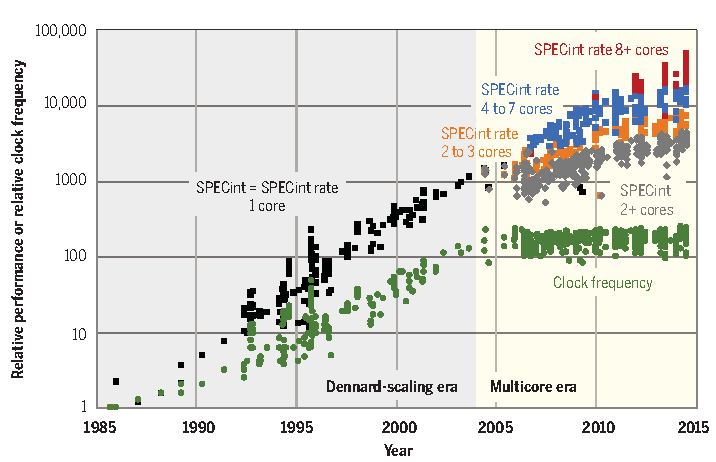
\includegraphics{figures/SPECint.pdf}
    \caption{SPECint、SPECint-rate 以及时钟频率的年际增长 \cite{doi:10.1126/science.aam9744}}
    \label{fig:specint}
\end{figure}

诚然,本研究提出的方法还有诸多不足。

其一,本研究在数据集和其相关评估过程方面存在一些局限性。虽然笔者相信本研究提出的框架具有普遍性,但截至目前,本研究只在不涉及纹理采样或多通道着色的片段着色器上验证了提出的方法。此外,本研究采用的、从Shadertoy收集的、用于验证本研究所提出方法的着色器,其可能和游戏等图形应用程序中的着色器在性能表现上有一定偏差。未来的工作中,如果能将性能测量和预测的框架进行小幅修改,以拓展到其它着色器类型(如顶点着色器、几何着色器甚至计算着色器等)的话,本研究提出的方法的普适性将会更上一个台阶。同时,为了降低和游戏等更广泛的图形程序中的着色器程序的性能特征偏差,如果将类似的着色器通过抓帧的方法截取和记录,并且收集整理成为数据集的话,将对着色器性能的理解有不小的帮助。在着色器之外,固定流水线资源以及其它和性能相关的因素也可以进一步加入讨论,以创建一个完整的、端到端的绘制和计算流水线黑盒性能模型。

其二,本研究的准确性仍然有进步空间。鉴于本研究收集到的性能数据,其变异系数均在3\%以下,故而本研究提出的预测器的准确性在理论上仍然有一定的改进空间。正如第 \ref{sec:challenge} 节所讨论的,有许多因素影响着着色器程序的性能。这些因素来自方方面面,并且可能会以相互交织的形式共同影响最终的性能表现。这样一来,当前采集的性能样本,其数量可能不足以充分训练本研究提出的模型。笔者认为,数据增强可能是一种可行的解决手段。例如,通过对着色器中的表达式进行有损失的强度削弱、或通过 IR 变换的方法首先对着色器进行变异,再使用变异后的变体来进行性能样本的增强,可能可以暴露更多对理解性能起到帮助的性能样本,并让本研究提出的模型训练的更加出色。此外,在 SPIR-V 指令追踪阶段,当前的指令追踪方法只记录了着色器程序全部线程调用后的总指令执行数目。如果将这里的记录方式变为逐线程记录的话,虽然指令追踪阶段的速度会大大下降,且可能面临存储和使用上的困难,但是这些额外的信息很可能可以帮助模型更好的挖掘线程之间影响性能的行为。这也是一种更细粒度的性能上下文信息。另一种提升模型性能表现的思路是,通过跨程序语言的多任务表示学习来提升待构造的着色器性能模型的表现。类似 GraphCodeBERT \cite{DBLP:conf/iclr/GuoRLFT0ZDSFTDC21}的预训练范式在本研究的工作中尚没有得到应用,但利用在其它语言上训练好的通用程序语言表示,再加以着色器专有的性能任务进行微调的方法,未尝不是一种可能的选择。

其三,作为数据驱动的方法,性能预测的可解释性仍然需要更多关注。具体到本研究,虽然本研究提出的预测模型能够以平台独立的方式,针对目标平台上运行的着色器程序提供相对准确的性能预测值,但是确定该着色器性能现状的瓶颈的问题仍然需要程序员自身的智慧。对此,笔者认为可行的一种改进是构造或实现一类在各个典型性能瓶颈方向上变异的着色器性能样本对,并在程序员需要优化建议时,通过让本研究提出的模型预测这些变化后的着色器的时间,来给出大致的瓶颈方向的参考。

除了以上这些局限之外,最近非常活跃的大语言模型领域也启发笔者,本研究提出的方法可能可以作为将性能数据加入解决程序任务的大模型中的一种方法。一种可能的想法是,通过将性能信息送入经过预训练的大模型中,这些大模型可能拥有以完全自动化的方式优化用户提供的着色器、并且解决用户所面临的软件性能问题的能力。

\bibliography{bib/main}

% \bibliography{bib/ustc}  % 参考文献使用 BibTeX 编译
% \printbibliography       % 参考文献使用 BibLaTeX 编译

% \appendix
% % !TeX root = ../main.tex

\chapter{补充材料}


\section{利用基座语言模型进行着色器类型标注时使用的提示词}
\label{sec:prompt_appendix}

{\added 使用基座语言模型进行着色器类型标注时,提示词的选择对标注的性能存在一定影响。本文主要探索了三种形式的基座语言模型提示词,分别为 \ref{lst:noPromptPrompt} 的无具体类别提示的提示词,\ref{lst:simplePromptPrompt} 的有简单类别提示的基座语言模型提示词,以及 \ref{lst:detailedPromptPrompt} 的有详细类别提示的基座语言模型提示词。}

\lstdefinestyle{plaintext}{
  language={},  % Resetting the language to prevent keyword styling
  basicstyle=\ttfamily\small,
  keywordstyle=\ttfamily\small,
  identifierstyle=\ttfamily\small,
  commentstyle=\ttfamily\small,
  stringstyle=\ttfamily\small,
  showstringspaces=false,
  breaklines=true,
  %frame=none,
  numbers=none
}

\begin{lstlisting}[style=plaintext, caption={无类别提示的基座语言模型提示词}, label=lst:noPromptPrompt]
You are a computer graphics specialist, and you are tasked to classify the following shaders.

The shader is as follows:
```
<shader>
    <pass type="image">
        此处填充着色器内容
    </pass>
    如果有其它渲染通道,此处将继续以 pass 标签的方式填充
</shader>
You MUST first explain your reason for your choice, then respond with xml format wrapped in a Markdown code block. The root element of the XML is result, and each tag is a tag element with a name attribute.
For example, here is an example code block for a shader labeled "2d" and "raytracing":
```
<result>
    <tag name="2d" />
    <tag name="raytracing" />
</result>
```
You have access to the following class tags:
- 2d
- 3d
- raytracing
- volume
- noise
- simulation
- material
- effects
Please FIRST give deductions step by step, and THEN give your answer. Your answer should be conservative.
\end{lstlisting}

\begin{lstlisting}[style=plaintext, caption={有简单类别提示的基座语言模型提示词}, label=lst:simplePromptPrompt]
(上面部分与无类别提示的基座语言模型提示词完全相同,省略)

You have access to the following class tags:
- 2d (Explaination: No 3D rendering techniques are involved in producing this image.)
- 3d (Explaination: 3D rendering techniques are used in producing this image.)
- raytracing (Explaination: Ray tracing (including ray marching) techniques are used in generating the intermediate or final image results in this shader.)
- volume (Explaination: Volumetric rendering techniques are used in generating this shader, or the generated effect are of volumetric.)
- noise (Explaination: Noise functions are used in generating the output or intermediate results of this shader. Including Fractal Brownian Motion (FBM), perlin, worley, simplex, blue noise and other noise functions.)
- simulation (Explaination: Simulation techniques are used in generating the output or intermediate results of this shader. Including fluld, diffusion, particle, dynamics or reaction simulations and automata, game-of-life simulations.)
- material (Explaination: Complex materials are present in the shader. This includes water, glass, metal, plastic and translucent materials, reflection and refraction behaviours, and PBR material models.)
- effects (Explaination: Postprocessing effects are used in the shader. This includes bloom, distortion, glitch, glow, blur, warp, dithering, filtering and other effects.)

Please FIRST give deductions step by step, and THEN give your answer. Your answer should be conservative.
\end{lstlisting}

    
\begin{lstlisting}[style=plaintext, caption={有详细类别提示的基座语言模型提示词}, label=lst:detailedPromptPrompt]
(上面部分与无类别提示的基座语言模型提示词完全相同,省略)

You have access to the following class tags:
- 2d (Explaination: No 3D rendering techniques are involved in producing this image.)
- 3d (Explaination: 3D rendering techniques are used in producing this image.)
- raytracing (Explaination: Ray tracing (including ray marching) techniques are used in generating the intermediate or final image results in this shader.)
- volume (Explaination: Volumetric rendering techniques are used in generating this shader, or the generated effect are of volumetric.)
- noise (Explaination: Noise functions are used in generating the output or intermediate results of this shader. Including Fractal Brownian Motion (FBM), perlin, worley, simplex, blue noise and other noise functions. However, the noise function should be non-trivial to implement.)
- simulation (Explaination: Simulation techniques are used in generating the output or intermediate results of this shader. Including fluld, diffusion, particle, dynamics or reaction simulations and automata, game-of-life simulations.)
- material (Explaination: Complex materials are present in the shader. This includes water, glass, metal, plastic and translucent materials, reflection and refraction behaviours, and PBR material models. However, Phong materials and pure lambertian reflections are generally not considered to be part of this class.)
- effects (Explaination: Postprocessing effects are used in the shader. This includes bloom, distortion, glitch, glow, blur, warp, dithering, filtering. However, simple effects like diffuse lighting, simple blur, or simple sharpening will not count.)

Please FIRST give deductions step by step, and THEN give your answer. Your answer should be conservative.
\end{lstlisting}

\section{SPIR-V 分词实现}

算法 \ref{alg:tokenizer} 展示了 SPIR-V 的分词过程。其中,TokenizeModule 函数在输出一个 \verb|[BOS]| 词元后,会获得该 SPIR-V 模块的入口函数和其引用的所有函数,并且将其顺序排列;之后,对于每个函数中的每条指令,TokenizeInst 会将其进行分词,并利用 PushToken 函数顺序输出词元。对于字符串、整数和浮点数字面值,分词器统一采用转换为字符串、增加 offset 进行原样输出的方法进行分词。

\begin{algorithm}
    % \SetAlgoLined %显示end
	\caption{SPIR-V 分词例程伪代码}%算法名字
    \label{alg:tokenizer}
\SetKwFunction{FTokenizeInst}{TokenizeInst}
\SetKwFunction{FTokenizeModule}{TokenizeModule}
\SetKwFunction{FTokenizeStringLiteral}{TokenizeStringLiteral}
\SetKwFunction{FPushToken}{PushToken}
\SetKwProg{Fn}{Function}{:}{}


\Fn{\FTokenizeStringLiteral{str}}{
    \ForEach{ch $\in$ str}{
        \tcc{PushToken($tok$) 用来输出一个词元 $tok$}
        \FPushToken{SymbolOffsets::ByteEncodedLiteralBegin + ch};
    }
}

\Fn{\FTokenizeInst{spirv\_inst}}{
    \FPushToken{SymbolOffsets::OpCodeBegin + spirv\_inst.opcode()}

    \ForEach{operand $\in$ spirv\_inst}{
        \uIf{isIdType(operand)}{
            \FPushToken{SymbolOffsets::IdBegin + operand.AsId()}\;
        }
        \uElseIf{isStringLiteral(operand)}{
            \FTokenizeStringLiteral{operand.AsString()}\;
        }
        \uElseIf{isIntegerLiteral(operand) or isFPLiteral(operand)}{
            \FTokenizeStringLiteral{to\_string(operand.AsNum())}\;
        }
    }
}

\Fn{\FTokenizeModule{spirv\_module}}{
    \tcc{首先输出一个 [BOS] 词元,[BOS] 词元在特殊符号中编号为 1}
    \FPushToken{SymbolOffsets::SpecialSymbolBegin + 1}\;
    \tcc{获得入口函数及其引用的所有函数的列表}
    funcs \gets spirv\_module.collectCallTreeFromRoots()\;
    \ForEach{f $\in$ funcs}{
        \ForEach{inst $\in$ f}{
            \FTokenizeInst{inst};
        }
    }
}
\end{algorithm}

\backmatter

\ifthenelse{\boolean{BlindReview}}{
  % No-op; won't include acks
}{
  % Not blind review; include the acks
  % !TeX root = ../main.tex

\begin{acknowledgements}

时光荏苒,日月如梭。转眼之间,我已经在科大度过了第七个年头。在科大,有幸结识了许多良师益友,在与他们的交往中,我不仅学习到了各种知识,还懂得了许多人生道理。

本研究的工作离不开黄亦铠同学的努力。黄亦铠同学完成了本研究中若干平台的测试和模型训练、部分新技术方案的探索和 Demo 的开发工作。同时,感谢何纪言同学分享对本研究所提出问题的独特视角。

感谢刘利刚老师。有幸在本科的图形学课程上结识刘利刚老师,并在图形和计算几何实验室度过了充实的三年。刘利刚老师深厚的学术功底,严谨的工作态度使我受益良多。衷心感谢刘利刚老师给予我的悉心教导和热情帮助。感谢总是出现在讨论班的陈发来老师,给予过我几何相关问题指导的傅孝明老师,以及在科大有幸结识和上过课的各位良师们。
% TODO: write some

感谢七年里结识的众多好友。感谢舍友和准舍友们,每天叫我去干饭,然后讨论天马行空的稀奇古怪问题;感谢图形和计算几何实验室一起学习的同学们,与他们的讨论让我受益良多。还有很多人想感谢,但是这里空太小,写不下,就让我在心里默默的记下来吧。

最后要感谢我的家人。是您们在二十四年来的陪伴和支持,让我能够安心学习和进步。感谢王志恒同学对我的关心和支持,很高兴能够遇见你。

% 在研究学习期间,我有幸得到了三位老师的教导,
% 他们是:我的导师,中国科大XXX研究员,中科院X昆明动物所马老师以及美国犹他大学的XXX老师。
% 三位深厚的学术功底,严谨的工作态度和敏锐的科学洞察力使我受益良多。
% 衷心感谢他们多年来给予我的悉心教导和热情帮助。

% 感谢XXX老师在实验方面的指导以及教授的帮助。
% 科大的XXX同学和XXX同学参与了部分试验工作,在此深表谢意。

\end{acknowledgements}

}
% !TeX root = ../main.tex

\begin{publications}

\section*{已发表论文}

\begin{enumerate}
\item A A A A A A A A A
\item A A A A A A A A A
\item A A A A A A A A A
\end{enumerate}

\section*{待发表论文}

\begin{enumerate}
\item A A A A A A A A A
\item A A A A A A A A A
\item A A A A A A A A A
\end{enumerate}

\section*{研究报告}
\begin{enumerate}
\item A A A A A A A A A
\item A A A A A A A A A
\item A A A A A A A A A
\end{enumerate}

\end{publications}


\end{document}
